
\documentclass{article}
\pdfoutput=1
\usepackage{arxiv}
\setcitestyle{authoryear,open={(},close={)}}
\renewcommand{\cite}{\citep}

\usepackage[utf8]{inputenc} %
\usepackage[T1]{fontenc}    %
\usepackage{hyperref}
\usepackage{url}
\usepackage{booktabs}       %
\usepackage{amsfonts}       %
\usepackage{nicefrac}       %
\usepackage{microtype}      %
\usepackage{dsfont}
\usepackage{graphicx}
\usepackage{amsmath}
\usepackage{mathtools}
\usepackage{amssymb}
\usepackage{amsthm}
\usepackage{cases}
\usepackage{color}
\usepackage{textcomp}
\usepackage{xcolor}
\usepackage{caption}
\usepackage{bbm}
\usepackage{comment}
\usepackage{xspace}
\usepackage{multirow}
\usepackage{subcaption}
\usepackage{authblk}
\usepackage{xspace}
\usepackage{algpseudocode}
\usepackage{adjustbox}
\usepackage{wrapfig}


\usepackage{microtype}
\usepackage{graphicx}
\usepackage{booktabs} %

\usepackage{hyperref}

\usepackage{amsmath}
\usepackage{amssymb}
\usepackage{mathtools}
\usepackage{amsthm}
\usepackage{mleftright}

\usepackage[capitalize,noabbrev]{cleveref}

\theoremstyle{plain}
\newtheorem{theorem}{Theorem}[section]
\newtheorem{proposition}[theorem]{Proposition}
\newtheorem{corollary}[theorem]{Corollary}
\newtheorem{definition}[theorem]{Definition}
\newtheorem{assumption}[theorem]{Assumption}
\theoremstyle{remark}
\newtheorem{remark}[theorem]{Remark}

\input{math_commands.tex}
\newcommand{\LC}{\texttt{LC}\xspace}
\newcommand{\Claude}{\text{Claude}}
\hypersetup{
    colorlinks,
    citecolor=[rgb]{0.00, 0.45, 0.70}, %
    linkcolor=[rgb]{0.01, 0.62, 0.45}, %
    urlcolor=[rgb]{0.68, 0.45, 0.63} %
}
\definecolor{green1}{rgb}{0.01, 0.62, 0.45}
\definecolor{blue1}{rgb}{0.00, 0.45, 0.70}
\definecolor{blue2}{rgb}{0.612, 0.8, 0.902}
\definecolor{purple1}{rgb}{0.68, 0.45, 0.63}
\definecolor{red1}{rgb}{1.0, 0.1, 0.3}
\definecolor{red2}{rgb}{1.0, 0.77, 0.80}

\usepackage{todonotes}
\usepackage{enumitem}
\newcommand{\E}{\mathbb{E}}
\newcommand{\LM}{\text{LM}}
\newcommand{\RL}{\text{RL}}
\newcommand{\SFT}{\text{SFT}}
\newcommand{\User}{\text{User}}
\newcommand{\Base}{\text{Base}}
\newcommand{\Para}{\text{Para}}
\newcommand{\LLM}{\text{LLM}}
\newcommand{\Sc}{R}
\newcommand{\NB}[1]{\textcolor{red}{(NB: #1)}}
\newcommand{\Lall}{\mathcal{L}_{\text{all}}}
\newcommand{\Lr}{\mathcal{L}_{\text{r}}}

\usepackage{amsmath}
\usepackage{amsthm}
\usepackage{amssymb}
\usepackage[bbgreekl]{mathbbol}

\DeclareMathSymbol\drule  \mathord{bbold}{"01}
\newcommand{\druleall}{{\drule_{\text{all}}}}
\newcommand{\drulel}{{\drule_{\mathcal{L}}}}
\newcommand{\phiCC}{\phi_{\text{cc}}}
\newcommand{\phiDC}{\phi_{\text{dc}}}
\newcommand{\DeltaAns}{\Delta^{|\mathcal{Y}|}}
\newcommand{\f}{f}
\newcommand{\reader}{reader}
\newcommand{\forecast}{\f(x, z)}
\newcommand{\surrforecast}{\widetilde{\f}(x, z)}

\usepackage{bbm}
% \usepackage[ruled]{algorithm2e}

\usepackage{wrapfig}
\usepackage{graphicx}
\usepackage{caption}
\usepackage{titletoc}
\usepackage{placeins}
\usepackage{graphicx}
\usepackage{placeins}
\usepackage[most]{tcolorbox} %
\usepackage{pdflscape}
\usepackage{algorithm}
\usepackage{tabularx}
\usepackage{siunitx}
\usepackage{soul}

\DeclareRobustCommand{\hlblue}[1]{{\sethlcolor{blue2}\hl{#1}}}
\DeclareRobustCommand{\hlred}[1]{{\sethlcolor{red2}\hl{#1}}}


\newcommand{\pms}[1]{\ensuremath{{\scriptstyle\pm #1}}}
\newcommand{\scr}[1]{\ensuremath{{\scriptstyle #1}}}

\newcommand*{\Chen}[1]{\textcolor{blue}{[Chen: #1]}}
\newcommand*{\edit}[1]{\textcolor{blue}{#1}}
\newcommand{\tnote}[1]{{\color{orange} [TM:#1]}}

\sisetup{detect-weight,mode=text}
\renewrobustcmd{\bfseries}{\fontseries{b}\selectfont}
\renewrobustcmd{\boldmath}{}
\newrobustcmd{\B}{\bfseries}
\usepackage[utf8]{inputenc} % allow utf-8 input
\usepackage[T1]{fontenc}    % use 8-bit T1 fonts
\usepackage{hyperref}       % hyperlinks
\usepackage{url}            % simple URL typesetting
\usepackage{booktabs}       % professional-quality tables
\usepackage{amsfonts}       % blackboard math symbols
\usepackage{nicefrac}       % compact symbols for 1/2, etc.
\usepackage{microtype}      % microtypography
\usepackage{xcolor}         % colors
\usepackage{amsmath}
\usepackage{amssymb}% http://ctan.org/pkg/amssymb
\usepackage{pifont}% http://ctan.org/pkg/pifont
\newcommand{\cmark}{\ding{51}}%
\newcommand{\xmark}{\ding{55}}%
\usepackage{xspace}
\usepackage{graphicx}
\usepackage{wrapfig}
% \usepackage{biblatex}
% \addbibresource{example_paper.bib}
\usepackage{algpseudocode}
\usepackage{color}
\usepackage{tabu}
\usepackage{diagbox}
\usepackage{float}
\usepackage{placeins}
\usepackage{multirow}
\usepackage{tikz}
% \usepackage{subfigure}
\usepackage{graphicx}
\usepackage{subcaption}
\usepackage{colortbl}
\usepackage{threeparttable}
% --- Stage badge: circled number matching Figure 3 ---
\definecolor{stepfill}{RGB}{20,20,20}   % near-black; set to {0,0,0} for pure black
\definecolor{cmtgray}{gray}{0.5}

\newcommand{\stepbadge}[1]{%
  \tikz[baseline=-0.55ex]{%
    \node[circle, fill=stepfill, text=white, inner sep=0pt,
          minimum size=1.15em, font=\sffamily\scriptsize\bfseries] {#1};}%
}
% ---- Global data structures (containers) ----
% To revert any of these to plain, just drop the \mathcal, e.g. \newcommand{\sctx}{C}
\newcommand{\sctx}{\mathcal{C}}   % shared context        (was C)
\newcommand{\tque}{\mathcal{T}}   % task queue            (was T)
\newcommand{\Lsto}{\mathcal{L}}   % summary backing store (was L)
\newcommand{\Rsto}{\mathcal{R}}   % raw backing store     (was R)

% ---- Ref-tag, renamed from r to avoid clashing with the result r_i ----
\newcommand{\reftag}{\rho}        % used as \reftag_{i,k}
% alternatives if you prefer: \newcommand{\reftag}{\mathrm{ref}}  or  {c}
% Right-aligned stage tag with optional gray description, e.g. \stage[note]{2}
\newcommand{\stage}[2][]{%
  \hfill
  \ifx\relax#1\relax\else
    \textcolor{cmtgray}{\itshape #1}\hspace{0.45em}%
  \fi
  \stepbadge{#2}%
}

% Lighter, italic comments for incidental notes
\renewcommand{\algorithmiccomment}[1]{\hfill\textcolor{cmtgray}{$\triangleright$\,\textit{#1}}}

% Prettier Input/Output labels (optional)
\algrenewcommand\algorithmicrequire{\textbf{Input:}}
\algrenewcommand\algorithmicensure{\textbf{Output:}}

% Highlight box for pluggable components
\definecolor{plugcolor}{RGB}{255,243,205} % soft amber
\newcommand{\plug}[1]{\colorbox{plugcolor}{#1}}
\definecolor{rowgray}{gray}{0.93}
\NewDocumentCommand{\yuzhen}{ mO{} }{\textcolor{red}{\textsuperscript{\textit{yuzhen}}\textsf{\textbf{\small[#1]}}}}
\newcommand{\toolName}{\textsc{DeLM}\xspace}
\newcommand{\revise}[1]{\textcolor{black}{#1}}
\definecolor{plugbg}{HTML}{DCEEFB}
\definecolor{plugfg}{HTML}{124780}
\DeclareRobustCommand{\plug}[1]{%
  {\setlength{\fboxsep}{1.5pt}%
   \colorbox{plugbg}{\textcolor{plugfg}{#1}}}}

\newtcolorbox{qualitativeBox}{
  colback=gray!10, %
  colframe=gray!20, %
  rounded corners, %
  boxrule=0.5pt, %
  left=10pt, %
  right=10pt, %
  top=5pt, %
  bottom=5pt, %
  boxsep=5pt, %
}
\newtcolorbox{ourMethodBox}{
  colback=blue1!10, %
  colframe=gray!20, %
  rounded corners, %
  boxrule=0.5pt, %
  left=10pt, %
  right=10pt, %
  top=5pt, %
  bottom=5pt, %
  boxsep=5pt, %
}
\newtcolorbox{theirMethodBox}{
  colback=red1!10, %
  colframe=gray!20, %
  rounded corners, %
  boxrule=0.5pt, %
  left=10pt, %
  right=10pt, %
  top=5pt, %
  bottom=5pt, %
  boxsep=5pt, %
}

\definecolor{gisttext}{HTML}{24292E}
\definecolor{gistbg}{HTML}{F4F6F8}
\definecolor{gistframe}{HTML}{CDD4DC}
\definecolor{gistfact}{HTML}{157F5F}
\definecolor{gistfail}{HTML}{C0392B}
\definecolor{gisttid}{HTML}{5A67B8}
\lstdefinestyle{gist}{%
  basicstyle=\footnotesize\ttfamily\color{gisttext},
  backgroundcolor=\color{gistbg},
  frame=single,
  framerule=0.7pt,
  rulecolor=\color{gistframe},
  framesep=7pt,
  framexleftmargin=7pt,
  xleftmargin=9pt,
  xrightmargin=5pt,
  breaklines=true,
  breakatwhitespace=false,
  columns=fullflexible,
  keepspaces=true,
  aboveskip=0.9\baselineskip,
  belowskip=0.7\baselineskip,
  emph={[1]FACT},emphstyle={[1]\bfseries\color{gistfact}},
  emph={[2]FAIL},emphstyle={[2]\bfseries\color{gistfail}},
  emph={[3]t0,t1,t2,t3,t4,t5},emphstyle={[3]\color{gisttid}},
}

\newtcolorbox{keyidea}{
  enhanced, breakable,
  colback=blue!8!white, colbacktitle=blue!8!white,
  colframe=blue!55!black, coltitle=blue!60!black,
  fonttitle=\bfseries\footnotesize,
  boxrule=0.6pt, arc=2pt, left=4pt, right=4pt, top=4pt, bottom=4pt
}

\begin{document}

\title{Decentralized Multi-Agent Systems with Shared Context}
\author{
    \large{Yuzhen Mao, ~
Azalia Mirhoseini}\linebreak
    \large{Stanford University}\linebreak
        {\texttt{\{yuzhenm,azalia\}@stanford.edu}}
}

\date{}

\maketitle

\begin{abstract}
Multi-agent systems (MAS) can scale large language model reasoning at test time by decomposing complex problems into parallel subtasks. However, most existing MAS rely on centralized orchestration, where a main agent assigns work, collects outputs, and merges results. As the number of subtasks grows, this controller becomes a communication and integration bottleneck. We propose Decentralized Language Models (\toolName{}), a MAS framework that decentralizes coordination through parallel agents, a shared verified context, and a task queue. Agents asynchronously claim subtasks, read accumulated progress, perform local reasoning, and write back compact verified updates. The shared context acts as a common communication substrate, enabling agents to build on one another’s verified progress without routing every update through a central controller. Empirically, \toolName{} improves both software-engineering test-time scaling and long-context reasoning. On SWE-bench Verified, \toolName{} achieves the best performance across Avg.@1, Pass@2, and Pass@4, with gains of up to 10.5 percentage points over the strongest baseline, while reducing cost per task by roughly 50\%. On LongBench-v2 Multi-Doc QA, \toolName{} achieves the highest average accuracy across four frontier model families, improving over the strongest baseline by up to 5.7 percentage points. The code is available on our project website at~\url{https://yuzhenmao.github.io/DeLM/}.
\end{abstract}
\section{Introduction}
\label{sec:intro}
\begin{figure}[!h]
    \centering
    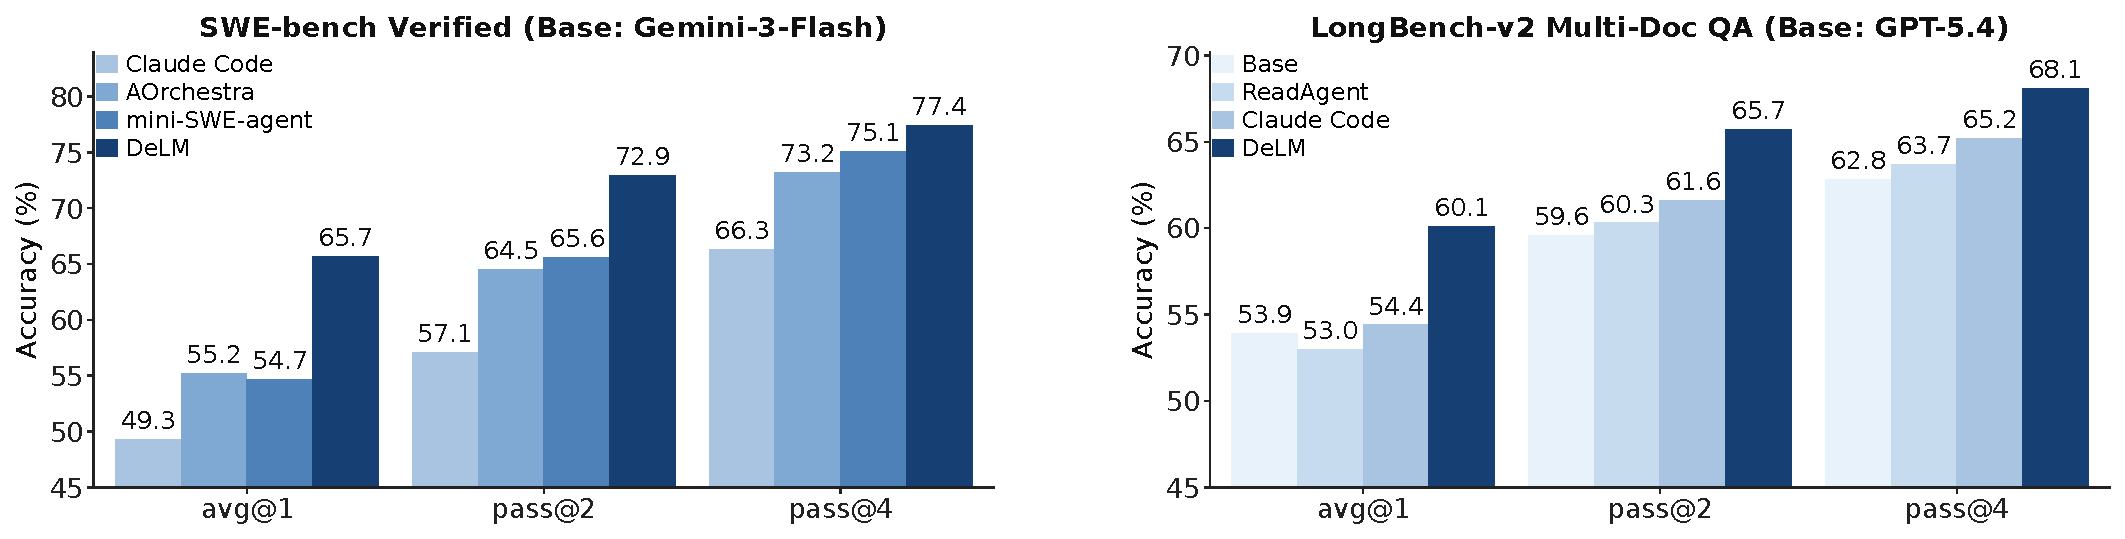
\includegraphics[width=1\linewidth]{teaser.pdf}
    \caption{\textbf{Comparison on SWE-bench Verified and LongBench-v2 Multi-Doc QA.} Our method, \toolName{}, achieves the best average performance across both agentic and long-context benchmarks.}
    \label{fig:placeholder}
\end{figure}


Multi-agent systems (MAS) offer a natural way to scale large language model reasoning at test time. Instead of relying on a single model invocation to solve a complex task end-to-end, MAS decompose the problem into subtasks, dispatch multiple agents in parallel, and aggregate their intermediate progress~\citep{hong2023metagpt, feng2026agentswing, ruan2026aorchestra, zhang2025recursive, openai_codex_2025, anthropic_claude_code_2026, team2026kimi}. This paradigm is increasingly important in two representative settings. The first is test-time scaling, where multiple agents can explore different hypotheses or pursue alternative reasoning paths in parallel while still sharing intermediate progress. The second is long-context reasoning, such as multi-document question answering, where agents can process different evidence clusters concurrently. In both cases, the value of MAS is not simply to issue more model calls, but to convert additional test-time computation into useful parallel progress. These two settings also capture core challenges in emerging automated research workflows~\citep{liu2026skydiscover,alphaevolve2025}, where agents must both scale exploration across hypotheses and reason over large collections of papers, code, experiments, and intermediate findings.
\begin{figure}
    \centering
    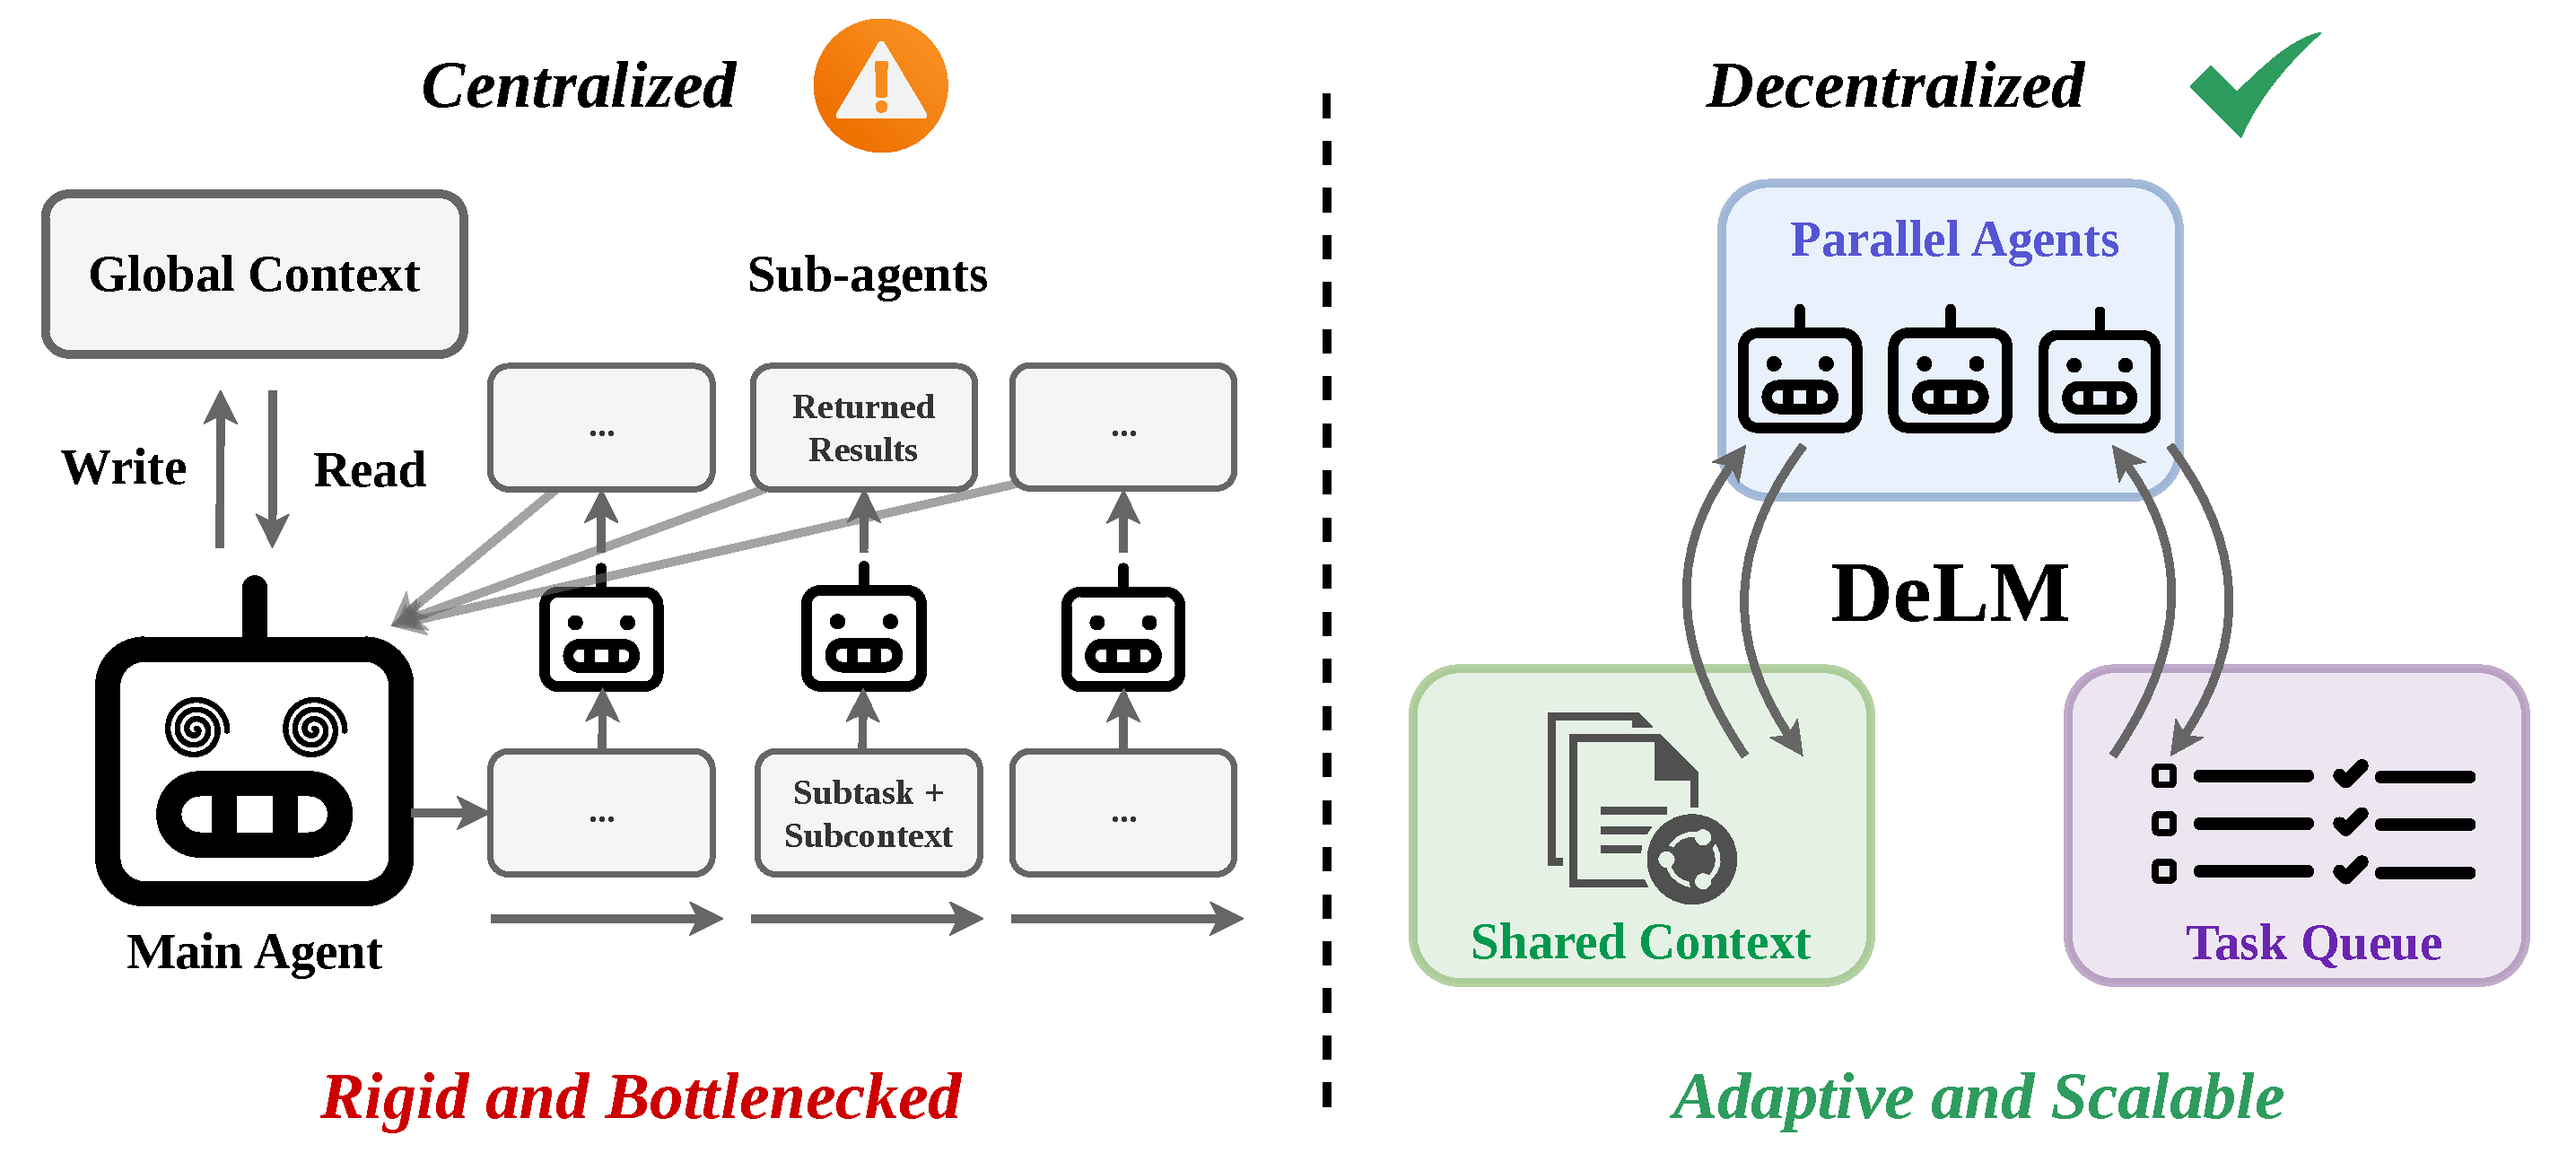
\includegraphics[width=1\linewidth]{first.pdf}
    \caption{
\textbf{Centralized vs. decentralized multi-agent systems.} Centralized MAS relies on a main agent to assign subcontexts, spawn sub-agents, and integrate returned results through a synchronous scatter--gather loop, creating a bottleneck where progress is gated by both the central merge step and the slowest worker. In contrast, \toolName{} decentralizes coordination through parallel agents, a shared context, and a task queue, allowing agents to exchange progress through shared state, asynchronously claim ready tasks, and scale more adaptively as the number of subtasks grows.
}
    \label{fig:first}
\end{figure}


Realizing this potential, however, depends critically on how agents coordinate. Most existing MAS frameworks, including Claude Code Subagents~\citep{anthropic_claude_code_2026}, Kimi Agent Swarm~\citep{team2026kimi}, and AOrchestra~\citep{ruan2026aorchestra}, rely on centralized orchestration: a main agent decomposes the problem, assigns subtasks and corresponding subcontexts to sub-agents, waits for their outputs, and then integrates the results or launches another round of subtasks, as illustrated in Figure~\ref{fig:first} (left). 
The limitation is that centralized MAS parallelize sub-agent execution, but not the coordination around it.
In test-time scaling, the benefit of additional agents depends on whether useful progress can be shared across workers efficiently and faithfully. Centralized orchestration weakens this benefit in two ways. First, it scales poorly: every useful finding, failure, or partial solution must return to the main agent, which then decides how to merge and broadcast that information to other sub-agents. As the number of agents grows, progress sharing becomes a serialized communication bottleneck. Second, during this routing process, the main agent may dilute, omit, or distort useful details, causing important progress to be lost. We provide a more detailed analysis in Section~\ref{sec:swe_analyze}. This bottleneck also arises in long-context reasoning: the main agent must pre-assign evidence clusters to sub-agents, often before knowing which evidence is relevant or how different pieces should be combined~\citep{anthropic_claude_code_2026, zhang2025recursive}. If a sub-agent receives insufficient context, it return control to the main agent, triggering additional retrieval or another delegation round. As subtasks or evidence clusters grow, this back-and-forth makes coordination slower, more iterative, and increasingly constrained by a single overloaded main agent.

To address these bottlenecks, we propose Decentralized Language Models (\toolName{}), a MAS framework that shifts coordination from a central controller to a shared problem state. As shown in Figure~\ref{fig:first} (right), \toolName{} is built around three core components: parallel agents, a shared context, and a task queue. Rather than routing every interaction through a main agent, agents asynchronously draw tasks from the queue, read accumulated progress from the shared context, perform local reasoning, and write back compact verified updates. This design also differs from peer-to-peer communication, where agents exchange messages directly. Instead, \toolName{} uses the verified shared context as a common communication substrate: once an update is admitted, it becomes visible to all agents as reusable problem state. As a result, \toolName{} supports both motivating settings: in test-time scaling, useful findings, failures, and partial solutions can propagate through shared context rather than being repeatedly merged and rebroadcast by a main agent. In long-context reasoning, agents can process different evidence clusters concurrently while maintaining a compact global view of the corpus and accumulated evidence.
\begin{keyidea}
\textbf{Key idea.} Unlike existing MAS, which rely on a central controller and synchronous scatter--gather coordination, \toolName{} lets agents coordinate asynchronously through a shared, verified context. Agents claim tasks from a queue and write back compact, verified results as they finish, making progress visible to all workers without requiring a main agent to merge, filter, and rebroadcast it.
\end{keyidea}

We evaluate \toolName{} in three settings that stress different forms of multi-agent coordination: (1) software-engineering test-time scaling on SWE-bench Verified~\citep{jimenez2024swebench}, which stresses parallel exploration across different reasoning trajectories; (2) long-context multi-document QA on LongBench-v2~\citep{bai2025longbench}, which stresses within-task parallelism as agents concurrently inspect different evidence clusters; and (3) aggregation-heavy long-context reasoning on OOLONG~\citep{bertsch2025oolong}, which highlights the complementarity between \toolName{}’s decentralized verified context and the code-mediated execution of RLM~\citep{zhang2025recursive}. Our key findings are: 
\begin{itemize}
    \item \textbf{\toolName{} converts parallel software-engineering attempts into shared exploration.} On SWE-bench Verified (\S~\ref{sec:swe}), as shown in Table~\ref{tab:swebench_verified}, \toolName{} achieves the strongest performance across test-time scaling metrics, reaching 77.4\% pass@4 while reducing cost to \$0.12 per task which is only roughly half of the baselines. Section~\ref{sec:swe_analyze} further explains these gains through trace-level examples showing how compact shared context helps agents reuse discoveries.
    \item \textbf{\toolName{} enables iterative shared-state reasoning over long contexts.} On LongBench-v2 (\S~\ref{sec:longbench}), as shown in Table~\ref{tab:multidoc_results}, \toolName{} achieves the highest average accuracy across four frontier models, improving over the best baseline by up to 5.7 percentage points. Section~\ref{sec:longbench_ablation} further shows that both admission-time verification and hierarchical summarization contribute to these gains.
    \item \textbf{\toolName{} acts as a coordination layer for programmatic reasoning systems.} On OOLONG (\S~\ref{sec:with_rlm}), as shown in Table~\ref{tab:oolong}, vanilla \toolName{} underperforms RLM because the benchmark requires exact row-level aggregation, where code-mediated execution is especially useful; however, combining RLM with \toolName{} yields the best accuracy and lowest cost, showing that \toolName{} extends beyond conversational agents to code-based reasoning workflows.
\end{itemize}

\section{Motivation and Design Principles}
\label{sec:motivation}

\subsection{From Prompt Routing to Shared State}

Section~\ref{sec:intro} identifies centralized coordination as a bottleneck in existing MAS. Here, we refine this observation by focusing on its communication mechanism. Centralized MAS are largely {prompt-routed}: intermediate progress is passed through the main agent, rewritten into subsequent prompts, and selectively exposed to other agents. Thus, parallel execution does not by itself guarantee parallel progress sharing.

This perspective motivates a different communication substrate. Instead of repeatedly encoding coordination decisions into prompts, \toolName{} makes intermediate progress persistent: agents write compact, verified updates into a shared context that later agents can read directly. Coordination therefore becomes {state-based}, with useful findings, failures, and constraints accumulating as shared problem state rather than passing through a central controller.

\subsection{Compact, Global, Unfoldable Shared Context}

State-based communication is useful only if the shared context remains usable as the problem grows. Sharing raw documents or full agent traces preserves maximal information, but quickly overwhelms each agent's context window and increases cost. Sharing only compact summaries is cheaper, but risks losing details, qualifications, or cross-document evidence needed for reliable reasoning.

\toolName{} addresses this trade-off with an unfolding mechanism. Agents read highly compact gists by default and selectively expand them into detailed summaries or raw evidence when needed. This coarse-to-fine access pattern enables coordination over the full problem while incurring detailed inspection costs only for relevant evidence.


\subsection{Verified Before Admission}

Because the shared context serves as the communication substrate for all agents, errors in this state can propagate widely. Once admitted, an unsupported claim may become reusable problem state, misleading later agents and shaping downstream reasoning. Post-hoc answer checking is insufficient, because such errors may have already influenced intermediate decisions.

\toolName{} mitigates this risk through admission-time verification. Before an update is added to the shared context, it is checked against its underlying evidence, including source context and reasoning trajectories. Unsupported or distorted updates are rejected or regenerated, turning the shared context from a raw message buffer into curated shared state.

\section{Decentralized Language Models (\toolName{})}
\label{sec:method}

\begin{figure}
    \centering
    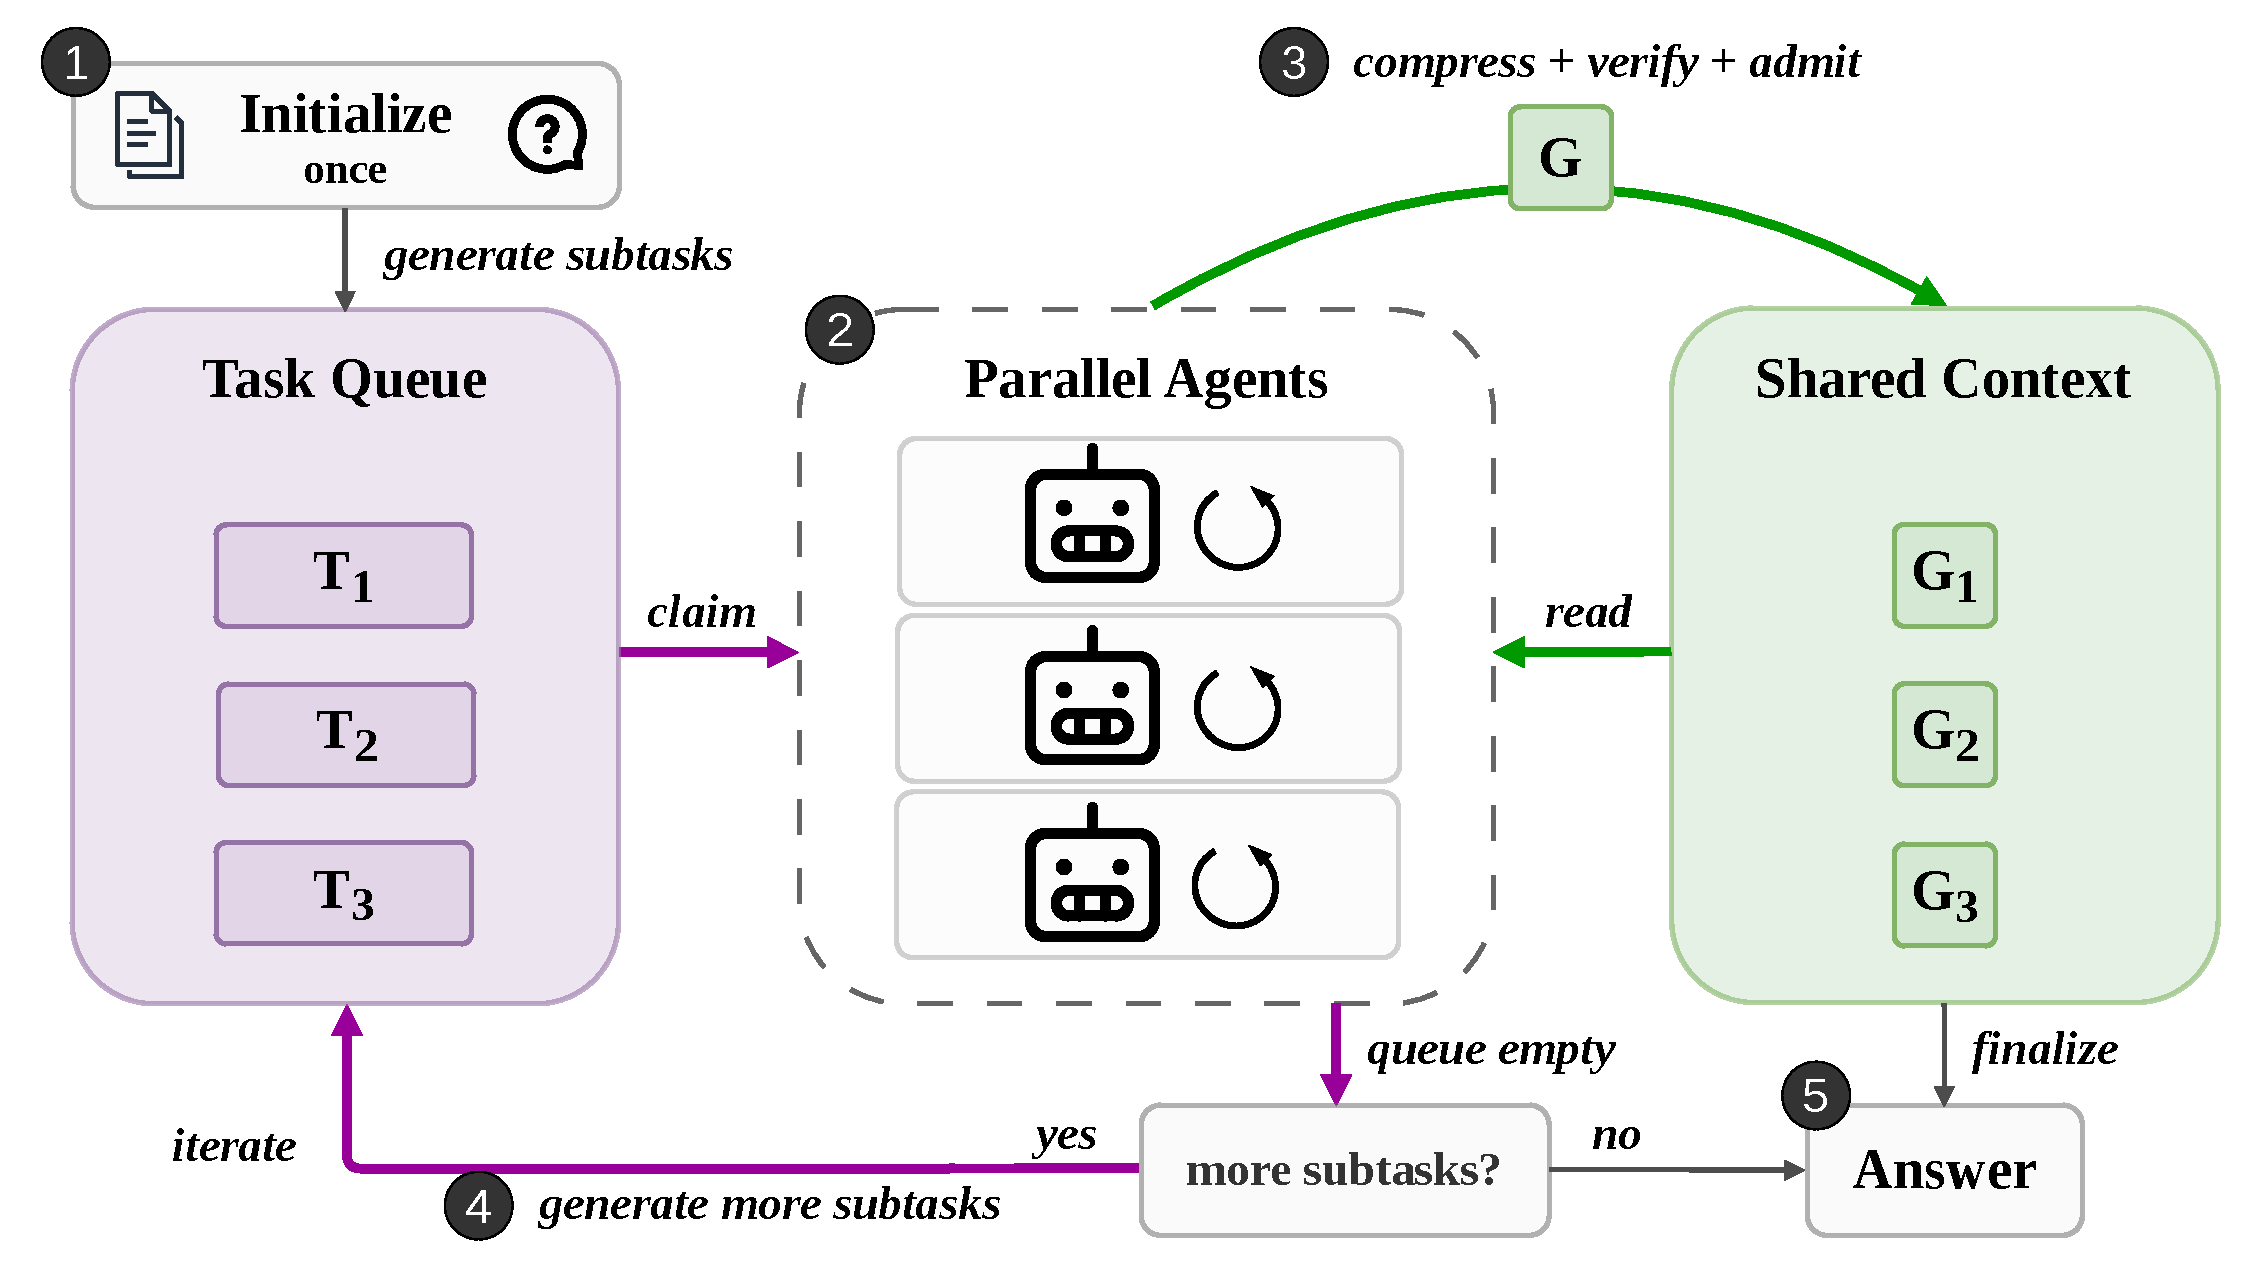
\includegraphics[width=1\linewidth]{pipe.pdf}
    \caption{\textbf{Overview of \toolName{}.} A one-time initialization step decomposes the input into initial subtasks and places them in a shared task queue. Parallel agents asynchronously claim tasks (${T_i}$), read the verified shared context, and perform local reasoning. Completed updates are compressed, verified, and admitted as compact gists ({${G_i}$}), making reusable progress visible to all agents. When the task queue becomes empty, the most recently completed agent checks the existing subtask states and shared context to decide whether additional subtasks are needed. If so, it generates and enqueues new tasks for another round of parallel execution; otherwise, it produces the final answer.
}
    \label{fig:pipeline}
\end{figure}

\begin{algorithm}
\caption{\textbf{\toolName{} pipeline.} \toolName{} maintains a shared context $\sctx$ and a task queue $\tque$. Agents execute queued subtasks in parallel, compress and verify their results $\{r_i\}$ into compact gists, admit verified gists to the shared context, optionally generate additional subtasks from accumulated state, and finally produce the answer from the verified shared context.}
\label{alg:dlm}
\begin{algorithmic}[1]
\Require Task $D$; optional source context $U$
\Ensure  Final answer $Y$

\State $\sctx \gets \emptyset$ \Comment{shared context}
\State $\tque \gets \Call{GenerateSubtasks}{D, U}$ \stage{1}

\Repeat
    \State $\{r_i\} \gets \Call{RunAgents}{\tque, \sctx}$ \stage[\Comment{execute subtasks in parallel}]{2}
    \State $\{G_i\} \gets \Call{CompressAndVerify}{\{r_i\}}$ \stage{3}
    \State $\sctx \gets \sctx \cup \{G_i\}$ \Comment{admit verified gists}

    \If{$\tque$ is empty}
        \State $\tque \gets \Call{GenerateMoreSubtasks}{D, \sctx}$ \stage{4}
    \EndIf
\Until{$\tque$ is empty}

\State $Y \gets \Call{Finalize}{D, \sctx}$ \stage{5}
\State \Return $Y$
\end{algorithmic}
\end{algorithm}

\toolName{} implements these design principles through two global structures: a shared context $\sctx$ and a task queue $\tque$. Given an input task $D$ and optional source context $U$, $\sctx$ stores compact, verified gists of accumulated progress, while $\tque$ stores pending subtasks for parallel execution.

As shown in Figure~\ref{fig:pipeline} and Algorithm~\ref{alg:dlm}, \toolName{} proceeds in five stages\mbox{: \stage{1}}~initialize the task queue from the input\mbox{, \stage{2}}~execute ready subtasks in parallel\mbox{, \stage{3}}~compress, verify, and admit updates into the shared context\mbox{, \stage{4}}~generate additional subtasks when the current shared context is insufficient, \mbox{and \stage{5}} produce the final answer once no further subtasks are needed. We next describe the two core mechanisms underlying this pipeline: Section~\ref{sec:shared_context} introduces the shared context and task queue, and Section~\ref{sec:compression_verification} describes how intermediate updates are compressed, verified, and admitted.

% This separation between a fixed loop and pluggable components is what makes \toolName{} modular: every \plug{highlighted} call site in Algorithm~\ref{alg:pipeline}---the summarizers $\phi_1, \phi_2$, the verifiers \textsc{Verify-U/T}, the planner \textsc{Plan}/\textsc{Replan}, the per-task worker \textsc{RunAgent}, and the finalizer \textsc{Finalize}---is a pluggable component that can be adapted to new domains without changing the pipeline.


\subsection{Shared Context and Task Queue}
\label{sec:shared_context}
\toolName{} maintains two global structures: a shared context $\sctx$ and a task queue $\tque$. The shared context stores compact, reusable problem state, including source evidence, completed subtask results, failed hypotheses, and intermediate constraints. The task queue stores pending subtasks that available agents can claim in parallel. Together, $\sctx$ and $\tque$ define the coordination interface: agents choose work from $\tque$ and communicate progress through admitted entries in $\sctx$.

The key design choice is that $\sctx$ contains gist entries $G_i$ rather than raw traces. Each gist summarizes information useful for future agents and points to more detailed evidence that can be retrieved through selective unfolding. Thus, every worker can read a lightweight global view of the current problem state without losing access to the underlying details.

The task queue determines how agents act on the shared state. Agents claim ready subtasks from $\tque$ asynchronously; after a gist is admitted into $\sctx$, later agents can build on the finding, avoid a falsified hypothesis, or reuse a partial solution without waiting for a central controller to redistribute it. When the queue is exhausted, the most recently completed agent uses the current subtask states and shared context to determine whether further subtasks are needed. If so, it generates and enqueues new subtasks conditioned on $\tque$ and $\sctx$; otherwise, it finalizes the answer from the accumulated shared state. Appendix~\ref{sec:orchestration} provides further details on dependency-aware
queueing, parallel execution, and systems optimizations


\subsection{Compression and Verified Admission}
\label{sec:compression_verification}
\toolName{} treats each shared-context update as an admission problem. Rather than writing raw agent outputs or unverified summaries directly into $\sctx$, it first compresses each completed result into a reusable gist and verifies that gist against its supporting evidence. Only updates that pass this gate become visible to other agents.

Specifically, given a completed result $r_i$, \toolName{} chooses the compression path based on the type of content being admitted. If $r_i$ is a reasoning trajectory, it may contain a successful finding, a falsified hypothesis, execution feedback, or a constraint for future agents. Since later agents usually need the distilled conclusion rather than the full trace, \toolName{} directly compresses $r_i$ into a gist $G_i$. If $r_i$ is a long source unit, however, direct gist-to-raw unfolding can be unreliable: the gist may not preserve enough detail to identify the exact raw span to unfold, while unfolding many candidate chunks to compensate is expensive. \toolName{} therefore uses a hierarchical path, $r_i \rightarrow S_i \rightarrow G_i$: it first constructs a reference-grounded summary $S_i$, then compresses $S_i$ into the compact gist $G_i$ admitted to $\sctx$. Both $S_i$ and the raw content remain in backing stores and can be recovered through selective unfolding. Appendix~\ref{sec:summarization} and Appendix~\ref{sec:unfold} give the full hierarchy and unfolding procedure, and Section~\ref{sec:longbench_ablation} validates this design through the ``No Hierarchical Summary'' ablation.


In operating-system terms, the gist layer functions as the small, always-resident working set visible to every agent, while $S_i$ and the raw store serve as backing storage. Selective unfolding acts like demand paging, loading finer-grained evidence into an agent's context only when the current subtask requires it.

Verification follows the same two paths. For a reasoning trajectory, \toolName{} checks whether the gist $G_i$ faithfully captures the relevant finding, failure, feedback, or constraint in $r_i$ using an LLM verifier. For a long source unit, verification is performed at both levels: the summary $S_i$ must be supported by the raw source, and the gist $G_i$ must preserve the supported claims and important qualifiers from $S_i$. Gists that pass are appended to $\sctx$ and become visible to later agents; gists that fail are rejected, regenerated with feedback. Appendix~\ref{sec:verification} gives the full admission-time verification procedure.

% This summarization procedure and admission-time gate turn the shared context from a raw message buffer into curated system state.
\section{Experiments}

\subsection{Experimental Setup}\label{sec:setup}
We first evaluate \toolName{} on two representative benchmarks that stress complementary aspects of multi-agent coordination: software-engineering test-time scaling and long-context multi-doc reasoning. Section~\ref{sec:with_rlm} later studies how \toolName{} can be combined with RLM~\citep{zhang2025recursive}.

(1) \textbf{SWE-bench Verified}~\citep{jimenez2024swebench}. A software-engineering benchmark built from real-world GitHub issues with human-verified task specifications and tests. We use it to evaluate agentic coding in realistic repository environments, where agents must inspect codebases, identify relevant files, implement fixes, and validate them through tests. This benchmark is especially suitable for our setting because its tasks require iterative exploration and coordination over large codebases rather than retrieving a single local answer.

(2) \textbf{LongBench-v2}~\citep{bai2025longbench}. A long-context benchmark designed to evaluate deep understanding and reasoning over realistic tasks. We focus on its multi-document QA setting, which contains 125 samples across diverse domains: Financial (15 samples), Government (23 samples), Multi-News (23 samples), Legal (14 samples), and Academic (50 samples). This setting is also suitable for our evaluation because its questions require multi-hop reasoning over evidence distributed across long contexts, rather than extracting a single local span.


We compare \toolName{} against different baselines. 
\textbf{Base} directly invokes the LLM once over the full input to produce an answer, without any decomposition or multi-agent orchestration. 
\textbf{Claude Code}~\citep{anthropic_claude_code_2026} is a tool-augmented agentic baseline that performs programmatic inspection and context compression to handle long inputs. \textbf{mini-SWE-agent}~\citep{yang2024sweagent} is a lightweight software-engineering agent that uses a simple linear agent loop with Bash as its primary interface.
\textbf{AOrchestra}~\citep{ruan2026aorchestra} is a centralized multi-agent system in which a main orchestrator dynamically creates specialized sub-agents on demand, instantiating each as a tuple of instruction, context, tools, and model to execute individual subtasks. 
\textbf{ReadAgent}~\citep{lee2024human} is an agentic long-context baseline that compresses the input into short gist memories and looks up the original passages when a subtask needs details the gists omit. For base models, we use Gemini 3 Flash~\citep{doshi2025gemini3flash} and Claude Opus 4.6~\citep{anthropic2026opus46} for the SWE-bench experiments; and GPT-5.4~\citep{openai2026gpt54}, Claude Sonnet 4.6~\citep{anthropic2025claude46sonnet}, Gemini 3 Flash, and DeepSeek-V4-Pro~\citep{deepseekai2026deepseekv4} for the LongBench-v2 experiments. 

All base models are evaluated through OpenRouter with default reasoning and sampling parameters. For Claude Code, we route the CLI through OpenRouter to support alternative base models and allow access to tools such as Read, Grep, and Bash. For AOrchestra, following the original configuration, we set \texttt{max-attempts = 10} for the orchestrator and \texttt{max-steps = 50} for each sub-agent. For ReadAgent, we set \texttt{min-lookup-pages = 1} and \texttt{max-lookup-pages = 6}, and use a 100-token gist budget, matching the gist budget used by \toolName{}.

\subsection{SWE-bench Verified}
\label{sec:swe}
SWE-bench Verified evaluates whether \toolName{} can improve test-time scaling in agentic software-engineering tasks. These tasks are largely sequential: each action depends on the outcome of the previous one, leaving little room to parallelize work {within} a single trajectory. Therefore, we scale {across} trajectories: we run each task $X$ times (with $X\in\{2,4\}$) and count it as solved if any one of the $X$ attempts yields a correct patch. We report three metrics: \textbf{Avg.@1} is the mean per-trial success rate, i.e., the expected accuracy of a single attempt; while \textbf{Pass@2} and \textbf{Pass@4} measure whether at least one of 2 or 4 attempts solves the task. 

Different methods use the same test-time scaling budget in different ways. For Base, mini-SWE-agent, Claude Code, and the original AOrchestra, we run $X$ independent attempts per task. Each trajectory starts from scratch and does not reuse intermediate discoveries from other attempts. We also introduce AOrchestra-Parallel, a variant built on AOrchestra. It starts each task once, but allows the main agent at each step to spawn up to $X$ subtasks and sub-agents in parallel, aggregate their outputs, and use the combined information to decide the next step. These parallel threads are therefore coupled through the main agent. \toolName{} uses the same agent harness as AOrchestra and likewise allows parallel threads to inform one another, but agents communicate through a verified shared context rather than through a central controller.
\begin{table}[t]
\centering
\setlength{\tabcolsep}{8pt}
\renewcommand{\arraystretch}{1.15}
\caption{Comparison on SWE-bench Verified across two base models. Best values are bolded.}
\label{tab:swebench_verified}
\begin{threeparttable}
\begin{tabular}{@{}l ccc | c@{}}
\toprule
\textbf{Method} & \textbf{Avg.@1} & \textbf{Pass@2} & \textbf{Pass@4} & \textbf{Cost/Task} \\
\midrule
\multicolumn{5}{@{}l}{\textit{Gemini 3 Flash}}\\
mini-SWE-agent       & 54.7\% & 65.6\% & 75.1\% & \$0.26 \\
Claude Code          & 49.3\% & 57.1\% & 66.3\% & --\,\tnote{a}    \\
AOrchestra           & 55.2\% & 64.5\% & 73.2\% & \$0.24 \\
AOrchestra-Parallel  & 56.4\% & 63.2\% & 71.8\% & \$0.25 \\
\rowcolor{rowgray}\textbf{\toolName{}} & \textbf{65.7\%} & \textbf{72.9\%} & \textbf{77.4\%} & \textbf{\$0.12} \\
\midrule
\multicolumn{5}{@{}l}{\textit{Claude Opus 4.6}}\\
mini-SWE-agent       & 76.9\% & 79.8\% & 81.7\% & \textbf{\$0.61} \\
Claude Code          & 76.1\% & 79.5\% & 81.3\% & \$0.69   \\
AOrchestra           & 74.7\% & 78.3\% & 80.1\% & \$0.70 \\
AOrchestra-Parallel  & 75.2\% & 78.1\% & 79.7\% & \$0.73 \\
\rowcolor{rowgray}\textbf{\toolName{}} & \textbf{78.0\%} & \textbf{80.7\%} & \textbf{82.5\%} & \$0.63 \\
\bottomrule
\end{tabular}
\begin{tablenotes}[flush]
\footnotesize
\item[a] The Claude Code CLI sends \texttt{cache\_control} blocks in the Anthropic API format, so cache reuse only works if the upstream provider honors those blocks. For Gemini-3-Flash the real cost without cache reuse is therefore around \$1 per task.
\end{tablenotes}
\end{threeparttable}
\end{table}

Table~\ref{tab:swebench_verified} shows that \toolName{} achieves the best performance across both base models. With Gemini 3 Flash, \toolName{} reaches 65.7\% Avg.@1, 72.9\% Pass@2, and 77.4\% Pass@4, outperforming all baselines on every metric. The largest gain appears in Avg.@1, where \toolName{} exceeds the strongest baseline, AOrchestra-Parallel, by 9.3 percentage points. At the same time, \toolName{} reduces cost to \$0.12 per task, roughly half the cost of the strongest agentic baselines. This shows that the improvement comes from using the same test-time budget more effectively, rather than from launching more trajectories or spending more tokens.

AOrchestra-Parallel improves Avg.@1 over the original AOrchestra, but performs worse on Pass@2 and Pass@4. This suggests that coupling parallel threads through a main agent can make attempts more consistent, but may also reduce exploration diversity.

The gains with Claude Opus 4.6 are smaller, likely because the base model is already strong and leaves less room for coordination to help. Even so, \toolName{} still achieves the highest accuracy across Avg.@1, Pass@2, and Pass@4, while remaining close to the lowest-cost method, only \$0.02 per task above mini-SWE-agent.

Overall, these results support our central claim: test-time scaling is more effective when parallel agents communicate through shared state. By making compact progress visible across trajectories, \toolName{} lets later agents avoid redundant exploration, build on prior findings, and focus on unresolved parts of the task. Section~\ref{sec:swe_analyze} analyzes these mechanisms through trace-level examples.
\vspace{-7mm}
\subsubsection{Why \toolName{} Is Both Accurate and Cost-Efficient on SWE-bench}
\label{sec:swe_analyze}
\vspace{-2mm}
% takeaway, and reorder
% First, parallel agents complement each other by sharing their failures and facts. Second, admitted constraints remain binding shared state instead of being softened or lost through a central controller. Third, compact patch summaries carry useful discoveries across threads without exposing every worker to long raw traces. 

Three trace-level mechanisms explain why \toolName{} improves both accuracy and cost efficiency. In the \toolName{} traces below, each shared entry is one thread's verified note, tagged with its thread id (\texttt{t0}, \texttt{t1}, \dots) and a type such as \texttt{FACT}, \texttt{FAIL}, or \texttt{PATCH\_SUMMARY}.

\vspace{-2mm}
\paragraph{(1) Parallel agents complement each other by sharing failures.}
The first mechanism is that failed hypotheses become reusable state rather than private dead ends. In isolated forks, a negative result remains local to one trajectory, so other attempts may spend their own budget rediscovering the same failure. In \toolName{}, once such a failure is admitted to the shared context, later agents can treat it as a constraint and redirect their search.

This mechanism appears in the trace below. The task fixes \texttt{lambdify} for single-element tuples. The natural guess, the Python printer layer, is a red herring; the real bug is on a separate tuple-building path in \texttt{sympy/\allowbreak utilities/\allowbreak lambdify.py}:

\begin{lstlisting}[style=gist]
[t0/FACT] AbstractPythonCodePrinter change did not affect lambdify output
[t1/FACT] sympy/utilities/lambdify.py:964 _recursive_to_string manual tuple join bypasses printer fix
[t0/FACT] sympy/utilities/lambdify.py:964 manual join for tuples lacks trailing comma logic
\end{lstlisting}
 
The load-bearing update is the negative result in the first line: thread \texttt{t0} shows that changing the printer does not affect the output. After reading this failure, \texttt{t1} avoids repeating the same detour and localizes the actual bypass in \texttt{\_recursive\_to\_string}; \texttt{t0} then records the concrete defect, the missing trailing comma. Thus, \toolName{} turns a failed hypothesis into shared progress, improving later agents' search efficiency.

\vspace{-2mm}
\paragraph{(2) Admitted constraints remain binding shared state.}
The second mechanism is that \toolName{} preserves important constraints as
shared state rather than routing them through a central controller. In centralized coordination, a main agent may soften, omit, or reopen constraints discovered by sub-agents before they can guide later work.
 
This mechanism appears in the trace below. Folding multiple search filters into one \texttt{.filter()} call is unsafe for multi-valued relations, where \texttt{.filter(A).\allowbreak filter(B)} and \texttt{.filter(A, B)} differ. In AOrchestra-Parallel, a sub-agent finds exactly this danger, but the constraint must pass through the main agent, which reopens the optimization and softens it into a tradeoff about reducing joins ``for many use cases''; the run fails. The relevant fact was found, but not preserved as binding state. In contrast, \toolName{} keeps the constraint explicit and reusable:
 
\begin{lstlisting}[style=gist]
[t3/FAIL] django/contrib/admin/options.py:1041 single .filter() breaks M2M multi-term search
[t3/FACT] Django ORM .filter(Q1, Q2) vs .filter(Q1).filter(Q2) differs for multi-valued relations
[t3/FACT] lookup_spawns_duplicates determines if single .filter() is safe
[t1/FACT] lookup_spawns_duplicates preserves M2M search semantics while optimizing FKs
\end{lstlisting}

Thread \texttt{t3} records the unsafe case (\texttt{FAIL}), the semantic reason, and the predicate \texttt{lookup\_spawns\_duplicates}, which determines when the optimization is valid. Thread \texttt{t1} then builds on this state to preserve M2M semantics while still optimizing foreign-key cases. Thus, later threads inherit the binding constraint rather than reopening a globally invalid simplification.


\paragraph{(3) Compact patch summaries carry discoveries.} 
The third mechanism is compact sharing, which lowers cost by preventing peer
communication from becoming another long raw transcript. Sharing full traces
would preserve information, but would also expose every worker to command
history, file dumps, failed edits, and intermediate reasoning. \toolName{}
instead shares a compressed version of the useful discovery, so later workers can reuse the result without reading the entire trajectory.

This mechanism appears in the trace below. Both the shared and no-share settings solve the task, but compact sharing reduces the cost from \$0.399 to \$0.125. The difference is not that \toolName{} shares more context; rather, it shares a compressed version of the useful search result (labeled as \texttt{PATCH\_SUMMARY}), which is generated by an LLM summarizer. One thread first rules out the ordinary tuple-printer path and localizes the actual bypass in \texttt{lambdify.py}:

\begin{lstlisting}[style=gist]
[t1/FACT] StrPrinter._print_tuple at sympy/printing/str.py:868 already includes trailing comma logic
[t1/FACT] sympy/utilities/lambdify.py:964 lacks trailing comma for single-element tuples
[t1/PATCH_SUMMARY] files=sympy/utilities/lambdify.py | idea=Modify _recursive_to_string to add a trailing comma for single-element tuples | evidence=reproduce_issue.py PASSED
\end{lstlisting}

This patch summary turns a multi-step debugging trajectory into a short,
evidence-backed handoff. Later workers do not need the full command history, file dumps, failed edits, or intermediate reasoning. Thus, compact sharing preserves the reusable discovery while avoiding the cost of exposing every peer to the raw trace, explaining why \toolName{} solves the task at much lower cost.

 
Together, these examples explain the trend in Table~\ref{tab:swebench_verified}: \toolName{} keeps reusable facts, failures, constraints, and patch summaries visible to all peers, while avoiding both redundant isolated search and the high token cost of raw trace sharing. This improves per-thread success while reducing cost.

\subsection{LongBench-v2 Multi-Doc QA}
\label{sec:longbench}
\begin{table}[t]
\centering
\setlength{\tabcolsep}{5pt}
\renewcommand{\arraystretch}{1.2}
\caption{Accuracy (\%) comparison on LongBench-v2 Multi-Doc QA across four base models. Results are mean$\pm$std over 3 independent runs. Numbers in parentheses denote the number of samples in each domain. Best values are bolded.}
\label{tab:multidoc_results}
\begin{tabular}{@{}l ccccc | c@{}}
\toprule
\textbf{Method} & \textbf{Fin.} (15) & \textbf{Govern.} (23) & \textbf{MNews} (23) & \textbf{Legal} (14) & \textbf{Acad.} (50) & \textbf{Avg.} \\
\midrule
\multicolumn{7}{@{}l}{\textit{GPT-5.4}}\\
Base & 62.2\tiny{$\pm$9.3} & 39.1\tiny{$\pm$1.7} & 50.5\tiny{$\pm$8.6} & {62.0}\tiny{$\pm$4.4} & 56.0\tiny{$\pm$1.2} & 53.9\tiny{$\pm$4.9} \\
Claude Code & {65.0}\tiny{$\pm$8.3} & 36.2\tiny{$\pm$2.0} & 50.7\tiny{$\pm$2.0} & 59.5\tiny{$\pm$3.4} & \textbf{60.7}\tiny{$\pm$0.9} & 54.4\tiny{$\pm$3.1} \\
ReadAgent & 
{57.8}\tiny{$\pm$3.9} & 34.8\tiny{$\pm$5.0} & 52.2\tiny{$\pm$8.7} & 
{61.9}\tiny{$\pm$4.4} &
58.0\tiny{$\pm$1.2} &
53.0\tiny{$\pm$3.3} \\
\rowcolor{rowgray}\textbf{\toolName{}} & \textbf{71.1}\tiny{$\pm$3.1} & \textbf{43.5}\tiny{$\pm$2.0} & \textbf{65.2}\tiny{$\pm$2.0} & \textbf{64.3}\tiny{$\pm$5.8} & {56.0}\tiny{$\pm$2.8} & \textbf{60.1}\tiny{$\pm$1.2} \\
\midrule
\multicolumn{7}{@{}l}{\textit{Claude Sonnet 4.6}}\\
Base & 68.9\tiny{$\pm$3.9} & 34.8\tiny{$\pm$1.1} & 46.4\tiny{$\pm$2.0} & 52.4\tiny{$\pm$3.4} & 64.0\tiny{$\pm$0.9} & 53.3\tiny{$\pm$1.9} \\
Claude Code & 66.7\tiny{$\pm$1.1} & 42.0\tiny{$\pm$2.0} & 47.8\tiny{$\pm$4.4} & 50.0\tiny{$\pm$3.4} & 52.0\tiny{$\pm$3.4} & 51.7\tiny{$\pm$2.4} \\
ReadAgent & 62.2\tiny{$\pm$3.9} & {44.9}\tiny{$\pm$4.4} & 43.5\tiny{$\pm$4.4} & 57.1\tiny{$\pm$4.1} & \textbf{64.7}\tiny{$\pm$2.3} & 54.5\tiny{$\pm$3.8} \\
\rowcolor{rowgray}\textbf{\toolName{}} & \textbf{73.3}\tiny{$\pm$3.1} & \textbf{46.4}\tiny{$\pm$2.0} & \textbf{55.1}\tiny{$\pm$2.0} & \textbf{59.5}\tiny{$\pm$3.4} & \textbf{64.7}\tiny{$\pm$0.9} & \textbf{59.8}\tiny{$\pm$1.5} \\
\midrule
\multicolumn{7}{@{}l}{\textit{Gemini 3 Flash}}\\
Base & {80.0}\tiny{$\pm$0.0} & 30.4\tiny{$\pm$0.0} & 43.5\tiny{$\pm$0.0} & \textbf{71.4}\tiny{$\pm$0.0} & 60.0\tiny{$\pm$2.3} & 57.1\tiny{$\pm$3.3} \\
Claude Code & 73.3\tiny{$\pm$3.1} & 26.1\tiny{$\pm$1.5} & 39.1\tiny{$\pm$0.0} & 57.1\tiny{$\pm$2.1} & 52.0\tiny{$\pm$1.9} & 49.5\tiny{$\pm$2.2} \\
ReadAgent & 75.6\tiny{$\pm$2.3} & 21.7\tiny{$\pm$4.4} & 46.4\tiny{$\pm$2.9} & 69.0\tiny{$\pm$3.4} & 62.0\tiny{$\pm$2.3} & 54.9\tiny{$\pm$1.1} \\
\rowcolor{rowgray}\textbf{\toolName{}} & \textbf{82.2}\tiny{$\pm$3.1} & \textbf{37.8}\tiny{$\pm$1.6} & \textbf{52.2}\tiny{$\pm$1.5} & \textbf{71.4}\tiny{$\pm$0.0} & \textbf{64.0}\tiny{$\pm$0.0} & \textbf{61.5}\tiny{$\pm$0.6} \\
\midrule
\multicolumn{7}{@{}l}{\textit{DeepSeek-V4-Pro}}\\
Base & \textbf{86.7}\tiny{$\pm$3.1} & 47.8\tiny{$\pm$2.0} & 44.9\tiny{$\pm$2.0} & \textbf{76.2}\tiny{$\pm$3.4} & 64.0\tiny{$\pm$0.9} & 63.9\tiny{$\pm$1.3} \\
Claude Code & 84.4\tiny{$\pm$3.1} & 36.2\tiny{$\pm$2.0} & 56.5\tiny{$\pm$4.4} & 64.3\tiny{$\pm$2.1} & 48.7\tiny{$\pm$0.9} & 58.0\tiny{$\pm$0.9} \\
ReadAgent & 71.1\tiny{$\pm$3.9} & 43.5\tiny{$\pm$4.4} & 30.4\tiny{$\pm$2.3} & 38.1\tiny{$\pm$4.1} & 50.7\tiny{$\pm$1.2} & 46.8\tiny{$\pm$1.8} \\
\rowcolor{rowgray}\textbf{\toolName{}} & \textbf{86.7}\tiny{$\pm$5.4} & \textbf{52.2}\tiny{$\pm$2.0} & \textbf{59.4}\tiny{$\pm$4.4} & 73.8\tiny{$\pm$3.4} & \textbf{65.3}\tiny{$\pm$0.9} & \textbf{67.5}\tiny{$\pm$1.2} \\
\bottomrule
\end{tabular}
\end{table}
LongBench-v2 Multi-Doc QA evaluates whether \toolName{} can improve evidence aggregation across long documents. Unlike SWE-bench Verified, where progress within one trajectory is largely sequential, this setting exposes substantial within-task parallelism: different agents can inspect different documents, identify complementary evidence, and contribute to a shared answer state.

As shown in Table~\ref{tab:multidoc_results}, \toolName{} achieves the highest average accuracy across all four model families: 60.1\% with GPT-5.4, 59.8\% with Claude Sonnet 4.6, 61.5\% with Gemini 3 Flash, and 67.5\% with DeepSeek-V4-Pro. Compared with the strongest baseline for each model family, these correspond to gains of 5.7, 5.3, 4.4, and 3.6 percentage points, respectively. \toolName{} also achieves the best or tied-best result in most domain-model combinations, suggesting that the benefit comes from a general improvement in evidence selection and reuse rather than from a single model or domain.

These gains come from first building a verified hierarchical view of the document set, enabling more targeted detailed inspection. \toolName{} first splits the input into chunks and uses a lightweight summarizer, DeepSeek-V4-Flash~\citep{deepseekai2026deepseekv4} by default, to produce hierarchical summaries. Verified gists are then admitted to the shared context, giving all agents a compact view of the corpus before they choose what to inspect in detail. This upfront global view helps agents identify cross-document connections, selectively unfold evidence, and avoid poorly targeted reading.

In contrast, centralized and programmatic-inspection baselines make more local inspection decisions, often from metadata, file names, or keyword matches before observing the relevant content. Early mistakes can therefore compound: a controller may inspect the wrong evidence, miss cross-document links, or require additional rounds of delegation. ReadAgent also uses gists, but its lookup process directly depends on lossy summaries, without hierarchical unfolding and admission-time verification. As a result, these baselines can cost less in long-context settings because they avoid the upfront cost of constructing and verifying a structured view of the full context. \toolName{} makes a different trade-off: it spends additional computation on hierarchical summarization and verification, but gains a more reliable understanding of the corpus, leading to more targeted evidence selection and higher prediction accuracy.

% \subsection{LongCoT-mini (Math and CS)}
% LongCoT-mini evaluates a complementary failure mode: rather than aggregating evidence across documents, the model must manage an extended reasoning trajectory that must be decomposed, checked, and recombined. Results are shown in Figure~\ref{fig:cot}. On Gemini-3-Pro, \toolName{} improves over the Base model from 18.0\% to 26.0\% on CS and from 26.3\% to 30.5\% on Math. On GPT-5.2, \toolName{} improves from 40.0\% to 47.0\% on CS and matches the strongest baseline on Math at 30.5\%. 

% These results suggest that the same shared-context construction extends beyond document-level evidence aggregation to intermediate reasoning traces. In this setting, verification is especially important: before an agent trace is summarized into an $G$ entry and admitted to $C$, \toolName{} checks whether its conclusion is well-supported. This prevents wrong local results from becoming shared premises, reducing error propagation across long reasoning trajectories.
% \begin{figure}[!h]
%     \centering
%     \begin{subfigure}{0.48\linewidth}
%         \centering
%         \includegraphics[width=\linewidth]{laa_cot_gemini.pdf}
%         \caption{Gemini-3-Pro Accuracy}
%     \end{subfigure}
%     \hfill
%     \begin{subfigure}{0.48\linewidth}
%         \centering
%         \includegraphics[width=\linewidth]{laa_cot_gpt.pdf}
%         \caption{GPT-5.2 Accuracy}
%     \end{subfigure}
%     \caption{Accuracy on LongCoT-mini for Gemini-3-Pro and GPT-5.2 across the CS and Math domains. \toolName{} achieves the highest accuracy in all four settings, while Claude Code and RLM show inconsistent gains relative to the single-agent base.}
%     \label{fig:cot}
% \end{figure}

% \subsection{Latency and Token Cost}\label{sec:cost}
% Figure~\ref{fig:latency} reports averaged latency and token consumption on the LongBench-v2 multi-document QA task. \toolName{} is slower than the plain Claude Code baseline due to additional overhead from summarization, verification, and shared-state management. However, it is substantially more efficient than RLM: latency decreases from 174.3s to 118.6s, making \toolName{} approximately $1.5\times$ faster, and token consumption decreases from 169K to 111K tokens, making it approximately $1.5\times$ more cost-efficient.

% This gap reflects differences in how context is explored. RLM plans and selects subcontexts based on limited signals, such as metadata or partial observations, before fully reading their content. When early selections are irrelevant or misaligned with the question, subsequent iterations compensate by exploring additional regions of the context, often up to the iteration limit, increasing latency and token usage. In contrast, \toolName{} allows agents to reason over a compact, content-aware representation before selectively unfolding only the necessary details. As a result, its retrieval is more targeted, reducing redundant exploration and improving overall efficiency.
% \begin{figure}[!h]
%     \centering
%     \includegraphics[width=0.99\linewidth]{latency_cost.pdf}
%     \caption{Latency and token consumption on multi-document QA. \toolName{} is $1.5\times$ faster and $1.5\times$ cheaper than RLM, while incurring overhead relative to the simpler Claude Code baseline due to its summarization, verification, and shared-context management.}
%     \label{fig:latency}
% \end{figure}
\vspace{-3mm}
\subsubsection{Which Components Make \toolName{} Effective on LongBench-v2}
\label{sec:longbench_ablation}

\begin{figure}[!h]
    \centering
    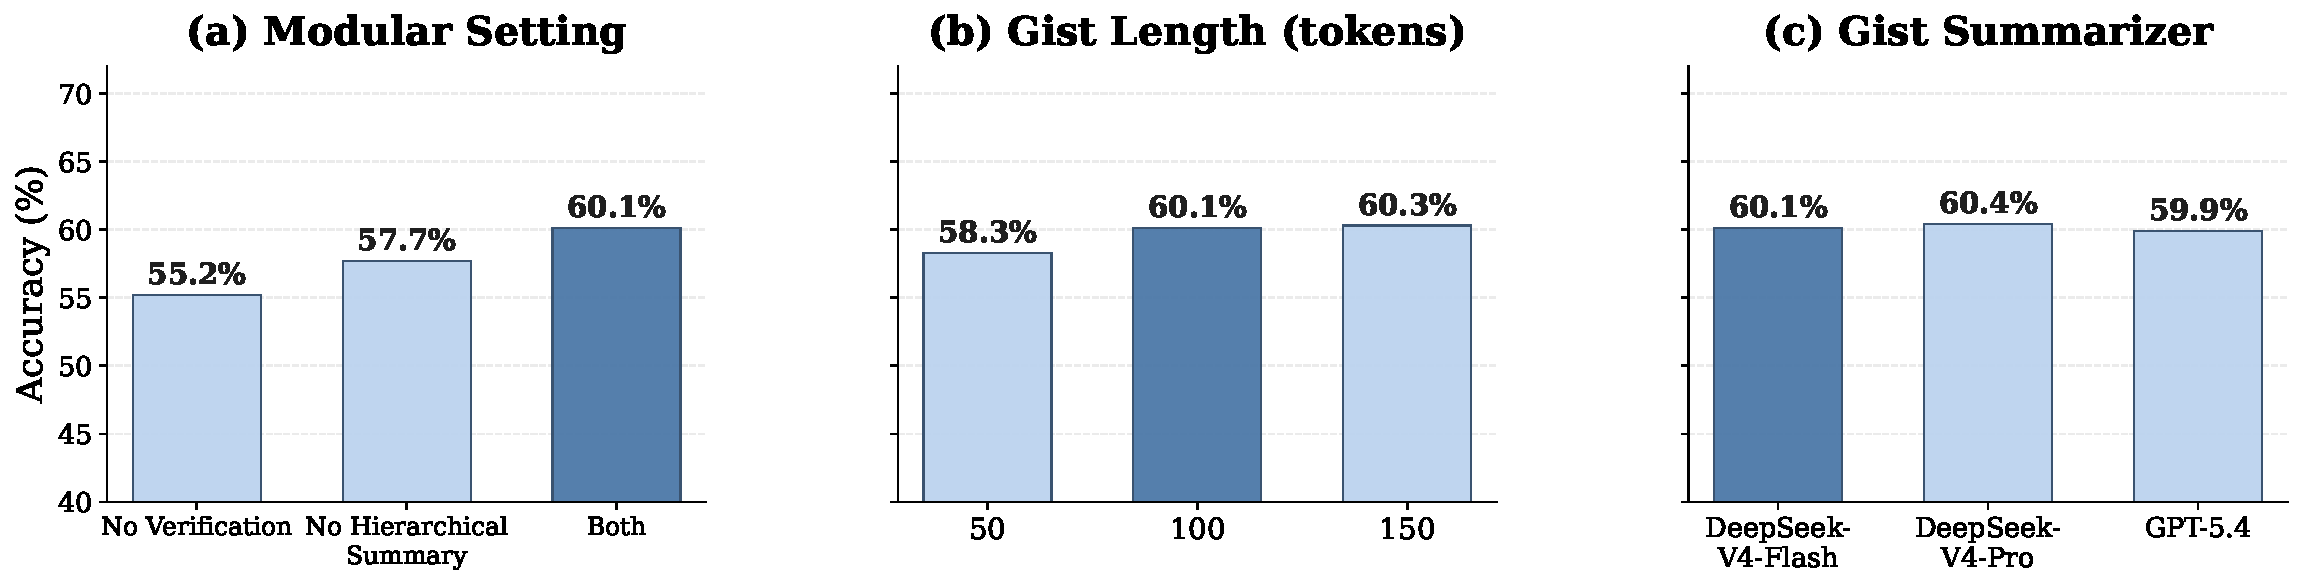
\includegraphics[width=1\linewidth]{ablation.pdf}
    \caption{\textbf{Ablation and robustness analysis on LongBench-v2 Multi-Doc QA.} All bars report accuracy averaged over the five domains with GPT-5.4. (a) Modular ablation: removing either the verification step or the hierarchical summary lowers accuracy. (b, c) \toolName{} is largely insensitive to its gist configuration: accuracy is stable once the gist is long enough (b) and across summarizers of varying cost (c). In every panel, the darker bar marks the default configuration used in Table~\ref{tab:multidoc_results}.}
    \label{fig:ablation}
\end{figure}
% \vspace{-3mm}
\paragraph{Modular ablation.}
To isolate the contribution of \toolName{}'s two core components, we remove admission-time verification and hierarchical summarization in turn, and report average accuracy over the five domains in Figure~\ref{fig:ablation}(a). Removing verification causes the largest drop, from 60.1\% to 55.2\%, showing that unsupported claims can corrupt downstream reasoning when they enter the shared context unchecked. Removing hierarchical summarization also hurts performance, lowering accuracy to 57.7\%, because gist-only routing provides a coarser path from global navigation to raw evidence. Thus, both components matter, with verification contributing the larger gain.

The trajectory evidence explains why the ``No Hierarchical Summary'' ablation degrades performance. Without the intermediate $S_i$ layer, \toolName{} must either route from a lossy gist directly to raw chunks or unfold many raw chunks to recover missing details. The PUMA EBIT query illustrates this failure mode. The document contains competing 2024 EBIT outlooks: an earlier range from the annual report and a later narrowed range from the H1 2024 interim report. The gist layer identifies candidate chunks, but the $S_i$ summary is what determines which source is later in time, localizes the relevant sub-chunk, and flags that the exact EBIT range must be recovered from raw evidence: (\texttt{S72.2} denotes the second segment of chunk 72, retrieved by scanning summary \texttt{S72}.)
\begin{lstlisting}[style=gist]
[t1] The later-in-time source is the H1 2024 interim report, which reiterates sales growth expectations and a narrowed EBIT outlook. The latest 2024 EBIT guidance is located in [S72.2].
[t1] However, the summaries do not provide the actual EBIT range values, so the precise latest target cannot be determined from summaries alone.
\end{lstlisting}

Only after this coarse-to-fine localization does the worker request raw evidence. The deep unfold then retrieves the precise anchored sub-chunk rather than the full report (\texttt{RAW} denotes the corresponding raw text recovered by unfolding):
\begin{lstlisting}[style=gist]
[S72.2 RAW] ... we narrow our outlook for the operating result (EBIT) to a range of EUR 620 million to EUR 670 million ...
\end{lstlisting}

This example shows why the hierarchy $G_i \rightarrow S_i \rightarrow \text{raw}$ is load-bearing. The gist supports cheap global navigation, the $S_i$ summary localizes the relevant raw span and detects when summary-level evidence is insufficient, and raw unfolding recovers the exact values. Removing the $S_i$ layer therefore weakens both evidence localization and cost-controlled reasoning, matching the performance drop in Figure~\ref{fig:ablation}(a).


The trajectory evidence also explains why removing verification hurts performance. In \toolName{}, agent outputs are not admitted into the shared context immediately; they must first be checked against their cited evidence. This prevents plausible but unsupported statements from becoming reusable shared state. In a legal question comparing \textit{Lucy v. Zehmer} and \textit{Texaco v. Pennzoil}, one agent introduced a specific damages claim that was not supported by its cited summary:
\begin{lstlisting}[style=gist]
[t2 OUTPUT] Pennzoil/Texaco is summarized as only conditionally affirmed, with punitive damages reduced from USD 3 billion to USD 1 billion [S5].
\end{lstlisting}
However, the cited gist only states that the case involved a conditional affirmance with remittitur; it does not contain the specific damages amounts. The verifier (an LLM) therefore rejects the update:
\begin{lstlisting}[style=gist]
[t2 VERIFY] WRONG: the claim that punitive damages were reduced from USD 3 billion to USD 1 billion is unsupported;[S5] only says there was a conditional affirmance with remittitur and gives no specific amounts.
\end{lstlisting}
After retry, the unsupported numerical claim is removed before the result is committed to $C$. Without this admission-time gate, the false detail would become available to later workers and the finisher as if it were grounded evidence, explaining the drop under the ``No Verification'' ablation in Figure~\ref{fig:ablation}(a).

\paragraph{Gist length.}
We vary the target gist length across 50, 100, and 150 tokens per source unit (Figure~\ref{fig:ablation}(b)). Accuracy improves from 58.3\% at 50 tokens to 60.1\% at 100 tokens, then plateaus at 60.3\% with 150 tokens. This suggests a threshold effect: once the gist is long enough to capture a source unit's relevance, additional length provides little benefit. We therefore use 100 tokens in the main experiments. Selective unfolding likely contributes to this stability, since agents can recover finer details from $S_i$ or the raw source when the gist is insufficient.

\paragraph{Summarization model.}
We also vary the gist summarizer ($\phi_2$, defined in \S~\ref{sec:summarization}), using DeepSeek-V4-Flash, DeepSeek-V4-Pro, and GPT-5.4 while keeping the rest of the pipeline fixed (Figure~\ref{fig:ablation}(c)). Accuracy remains nearly unchanged across the three summarizers (60.1\%, 60.4\%, and 59.9\%, respectively), with the cheapest model, DeepSeek-V4-Flash (our default), matching the stronger alternatives. Thus, a lightweight summarizer is sufficient for constructing the shared context, allowing \toolName{} to reserve stronger models for subtask reasoning without sacrificing accuracy.

\section{Combining \toolName{} with RLM}\label{sec:with_rlm}
Recursive Language Models (RLMs)~\citep{zhang2025recursive} process long contexts by recursively selecting context segments, issuing sub-calls, and composing the resulting partial answers. Crucially, RLM performs this process through a code-mediated Read-Eval-Print Loop (REPL): the long input is stored as an external variable that the model can inspect, parse, and aggregate programmatically. This makes RLM a natural fit for OOLONG~\citep{bertsch2025oolong}, an aggregation-heavy benchmark where each sample consists of timestamped, user-attributed entries and answering a question often requires classifying many entries before computing a distributional answer.

\begin{wraptable}{r}{0.5\textwidth}
\centering
\begin{tabular}{lcc}
\toprule
\textbf{Method} & \textbf{Acc.} & \textbf{Cost/Task} \\
\midrule
\multicolumn{3}{l}{\textit{OOLONG}} \\
RLM & 56.0\% & \$0.43 \\
\toolName{} & 53.3\% & \$0.47 \\
\toolName{}+RLM & \textbf{64.0\%} & \textbf{\$0.40} \\
\midrule
\multicolumn{3}{l}{\textit{LongBench-v2 Multi-Doc QA}} \\
RLM & 55.8\% & \$0.29 \\
\toolName{} & 57.9\% & \$0.30 \\
\toolName{}+RLM & \textbf{60.3\%} & \textbf{\$0.24} \\
\bottomrule
\end{tabular}
\caption{Comparison of RLM, \toolName{}, and their hybrid on LongBench-v2 Multi-Doc QA and OOLONG using GPT-5.}
\label{tab:oolong}
\end{wraptable}

We first evaluate \toolName{} and RLM separately on both LongBench-v2 Multi-Doc QA and OOLONG using GPT-5 with medium reasoning (RLM uses GPT-5-mini for sub-calls and recursion depth=1). As shown in Table~\ref{tab:oolong}, the two methods have complementary strengths. On LongBench-v2, \toolName{} achieves higher average accuracy than RLM at roughly the same cost per task. On OOLONG, however, \toolName{} underperforms RLM in both average accuracy and cost. This is because OOLONG is closer to a structured data-processing benchmark than a conversational reasoning benchmark (such as LongBench-v2): many questions require exact counting, filtering, comparison, and tie handling. In this setting, the natural-language shared context used by \toolName{} is not reliable. RLM performs better because its core interface is code-mediated: through a REPL environment, the model can inspect, parse, transform, and aggregate the input using executable programs and programmatic sub-calls. However, RLM still relies on centralized coordination, where recursive calls report back to a root process that must reconcile and aggregate their outputs. This centralized aggregation is less suitable for natural-language multi-document reasoning, helping explain RLM's weaker LongBench-v2 performance. These results motivate a hybrid design that combines RLM's precise REPL-based execution with \toolName{}'s decentralized coordination.

We therefore combine the two methods by retaining RLM as the underlying reasoner while adding two \toolName{} components: a verified shared context and a decentralized task queue. In this hybrid setting, there is no main-agent/sub-agent hierarchy; all agents are equally ranked RLM instances that coordinate through shared state. An initial RLM call produces a compact work plan, after which subtasks are placed into the task queue and claimed by parallel RLM workers. Each worker's output is admitted into the shared context only after passing the verification gate. The system then generates any additional subtasks from the current problem state, and computes the final answer from the verified shared context once no further subtasks are needed. This design preserves RLM's strength in precise code-mediated execution while adding \toolName{}'s decentralized coordination. As shown in Table~\ref{tab:oolong}, the combined method achieves the best accuracy and lowest cost on both benchmarks, indicating that RLM and \toolName{} are complementary rather than competing approaches.
\section{Related Work}
\label{sec:related_work}
\paragraph{Multi-Agent Systems.}
Recent LLM-based multi-agent systems improve task performance by decomposing problems across specialized or interacting agents. Early frameworks such as CAMEL~\citep{li2023camel} instantiate role-playing agents to study autonomous cooperation. MetaGPT~\citep{hong2023metagpt} and ChatDev~\citep{qian2024chatdev} further structure collaboration through software-engineering-inspired roles, communication protocols, and standardized workflows, demonstrating that specialization can reduce coordination complexity in multi-step tasks. AOrchestra~\citep{ruan2026aorchestra} dynamically creates task-specific sub-agents by instantiating their instructions, context, tools, and models; ToolOrchestra~\citep{su2025toolorchestra} trains a lightweight orchestrator to coordinate models and tools under accuracy, efficiency, and user-preference rewards; Squeeze Evolve~\citep{maheswaran2026squeeze} routes different stages of evolutionary inference to models of different cost and capability; and RecursiveMAS~\citep{yang2026recursive} replaces text-level communication with recursive latent-state transfer across agents.
Combee~\citep{li2026combee} also identifies centralized aggregation as a bottleneck under high parallelism, but focuses on scaling parallel prompt learning rather than decentralized agent coordination. Recent blackboard-style MAS~\citet{han2025exploring, salemi2025llm} use a shared board to let agents exchange messages or volunteer information, either for general reasoning or for data discovery.

These systems show that agent coordination can be scaled through dynamic delegation, learned orchestration, model routing, recursive collaboration, and shared blackboards. However, the orchestration-based methods primarily optimize how agents are created, routed, or composed, leaving the communication substrate itself unverified: intermediate outputs are passed, summarized, or aggregated without grounding each entry in its underlying evidence before downstream reuse; the blackboard-based methods write raw or lightly structured messages to the board and still route coordination through a selection step or a central poster. In contrast, \toolName{} treats the shared context as curated, verified state: agents coordinate fully asynchronously through a task queue with no central controller, every entry is admitted only after verification against its supporting evidence, and entries are stored as compact gists that unfold to finer detail on demand, keeping the shared state both reliable and scalable as the number of agents grows.

\paragraph{Programmatic Agentic Systems.}
A closely related class of systems equips language models with programmatic interfaces to external environments, enabling them to inspect state, invoke tools, manipulate artifacts, and recursively delegate computation. Recursive Language Models (RLMs)~\citep{zhang2025recursive} apply this paradigm to long-context reasoning by treating the prompt as an external environment and recursively selecting snippets for inspection. It performs this process through a code-mediated Read-Eval-Print Loop (REPL). Agentic coding systems such as Claude Code~\citep{anthropic_claude_code_2026} and Codex~\citep{openai_codex_2025} extend this idea to software environments, allowing models to read repositories, edit files, execute commands, and incorporate tool feedback. These approaches demonstrate that coupling language models with executable environments substantially enhances capability beyond single-pass generation. 

However, programmatic access alone does not solve the coordination problem. In many systems, planning is still routed through a main agent or local tool loop, and intermediate results are reused as raw observations or prose summaries without an admission-time grounding step. As a result, useful discoveries may remain local to one trajectory, while unsupported claims or softened constraints can propagate through later reasoning. \toolName{} is complementary to these systems: it does not replace tools, code execution, or REPL-style inspection, but provides a decentralized coordination layer in which tool-derived findings, failures, and partial solutions can be compressed, verified, and shared across agents. This complementarity is reflected in our OOLONG experiments (\S~\ref{sec:with_rlm}), where combining \toolName{} with RLM improves over either method alone.

\paragraph{Long-context LM systems.}
Another line of work addresses long-context reasoning by storing, compressing, or retrieving information beyond the model's current context window. \citet{mu2023learning} introduce a training-based approach that compresses long prompts into compact ``gist'' representations. Context-Folding~\citep{sun2025scaling} keeps long interactions within the context window by periodically compressing the conversation history. These methods reduce context length, but once fine-grained information is discarded, it cannot be reliably recovered when later reasoning requires precise details. ReadAgent~\citep{lee2024human} instead pairs compression with retrieval: it summarizes pages of text into short gist memories and looks up the original passages when a task needs details the gists omit. However, because lookup is triggered from lossy gists, ReadAgent can miss evidence whose relevance is not preserved in the compressed representation. 

Memory-augmented systems such as LongMem~\citep{wang2023augmenting}, MemGPT~\citep{packer2023memgpt}, Mem0~\citep{chhikara2025mem0}, and MemOS~\citep{li2025memos} introduce external memory mechanisms for LLMs to retain information across long interactions or task histories. For instance, MemGPT~\citep{packer2023memgpt} proposes an operating-system-inspired virtual context mechanism to decide what to keep in the active context and what to move into external memory. These systems make memory persistent, but retrieval is usually flat: a memory item is either selected into context or omitted. \toolName{} instead organizes shared information by abstraction level. Agents first reason over compact verified gists across the full problem, then selectively unfold relevant entries into detailed summaries and raw evidence. This hierarchy makes the shared context both global and recoverable.


\vspace{-2mm}
\section{Limitations and Future Work}\label{sec:limit}
\vspace{-1mm}
While our results demonstrate the effectiveness of \toolName{}, several directions remain open for future exploration. First, admission-time verification trades a modest amount of overhead for stronger reliability guarantees; lighter-weight verifiers, including learned models or rule-based checks for common claim types, could further improve efficiency while preserving the grounding benefits we observe. Second, \toolName{} inherits the decomposition quality of agents. Overly coarse decompositions leave agents with under-specified subtasks, while overly aggressive decompositions can spawn unnecessary agents and overcomplicate reasoning. A promising direction is to train adaptive agents that decide when to split, merge, or terminate subtasks based on the shared context. Third, as noted in prior work~\citep{zhang2025recursive}, there is no universally optimal prompt across models; different model families may require tailored prompts to elicit the intended behavior. Combining \toolName{} with prompt-evolution methods such as GEPA~\citep{agrawal2025gepa} could further adapt its decomposition, summarization, and verification prompts to each model family.

Beyond the benchmarks studied here, \toolName{} suggests a promising direction for automated research systems~\citep{alphaevolve2025, liu2026skydiscover}. Research workflows naturally combine test-time scaling with long-context reasoning: agents must explore alternative hypotheses, inspect large collections of papers or experimental logs, compare evidence across sources, and iteratively refine conclusions. A decentralized shared context could make such systems more efficient by preventing agents from repeatedly reading the same papers or rerunning the same failed analyses; more effective by allowing useful findings to propagate across parallel research threads; and more robust by admitting only verified claims into the shared state. We therefore view automated research as a natural application domain for future decentralized MAS.

\vspace{-2mm}
\section{Conclusion}
\vspace{-1mm}
We introduce \toolName{}, a decentralized multi-agent system in which agents coordinate through a shared context and task queue rather than a central controller. By admitting only compact, verified updates into shared state, \toolName{} turns intermediate progress into reusable problem state: agents can build on prior findings, avoid repeated failures, preserve constraints, and recover detailed evidence only when needed. On SWE-bench Verified, \toolName{} improves test-time scaling by making discoveries and failures reusable across parallel attempts, achieving higher pass rates while reducing cost. On LongBench-v2 Multi-Doc QA, \toolName{} improves long-context reasoning by constructing a verified, hierarchical view of the corpus, leading to higher accuracy. We further show that \toolName{} is complementary to RLM, where decentralized validated state improves programmatic aggregation. These results suggest that scalable multi-agent systems require not only more parallel agents, but also a reliable communication substrate for sharing progress across them.


\section{Acknowledgments}
We thank Shayan Talaei, Jon Saad-Falcon, Jacky Kwok, Hermann Kumbong, Ishan Khare, Miria Feng, Qizheng Zhang, Swapnil Gandhi, Michael Y. Li, Chun Deng, Chong Zeng, Rui Li, Ke Li, Marquita Ellis, Hangoo Kang, Adrian Gamarra Lafuente, Charles Ding, Tarun Suresh, Ziyu Chen, Zhuohan Gu, Yize Liu, and Ligeng Zhu. We would also like to thank our collaborators at the Stanford Artificial Intelligence Laboratory (SAIL) and Stanford HAI.

We gratefully acknowledge support from federal sources: NSF under No. 24-554 (AIMing) and DARPA under No. HR00112520038 (Fallingwater). We also gratefully acknowledge support from Stanford HAI, IBM (Code Generation), Lightspeed, Google, and Google DeepMind.
\newpage



\bibliography{bibliography}
\bibliographystyle{plainnat}


\newpage
\appendix
\onecolumn

\onecolumn
\section*{\LARGE Supplementary Material}
\label{sec:appendix}

% \section{Full Pipeline Pseudo-code}
% Algorithm~\ref{alg:dlm} in the main text presents a phase-level overview. Below, we give the full pseudo-code in Algorithm~\ref{alg:pipeline-full}.
% Each source unit $u \in \mathcal{U}$ and each agent reasoning trace $\Rsto$ contributes an entry to this shared context $\sctx$ through a hierarchical transformation. Specifically, a first-stage summarizer $\phi_1$ produces a reference-grounded summary $S$, and a second-stage summarizer $\phi_2$ further compresses $S$ into a highly compact gist $G$. Only $G$ is admitted to $\sctx$, while $S$ and the raw content are retained in addressable stores $\mathcal{L}$ and $\mathcal{R}$ to support later selective unfolding. Verification is enforced at the moment $S$ and $G$ are produced, ensuring that only verified gists enter $\sctx$. 

% The code will be released upon acceptance.

% \begin{algorithm}[!h]
% \caption{\toolName{} pipeline. \plug{Highlighted} components are pluggable (see \S\ref{sec:method}, second paragraph).}
% \label{alg:pipeline-full}
% \begin{algorithmic}[1]
% \Require Question $Q$; optional source units $\mathcal{U}$ (default $\emptyset$)
% \Ensure Final answer $Y$
% \Statex \textit{$\sctx$---shared context; $\mathcal{L},\mathcal{R}$---per-entry stores for $S$ and raw; $\mathcal{T}$---task queue; $\ell$---labels for $u, t$.}
% \State $C \leftarrow [\,]$;\ \ $\mathcal{L}, \mathcal{R} \leftarrow \emptyset$

% \If{$\mathcal{U} \neq \emptyset$}
%     \ForAll{$u \in \mathcal{U}$ \textbf{in parallel}}\Comment{seed: summarize, verify, and admit each source}
%         \State $S \leftarrow$ \plug{$\phi_1$}$(u;\, Q, C)$;\ \ $G \leftarrow$ \plug{$\phi_2$}$(S;\, Q, C)$ with \plug{\textsc{Verify-U}}$(G, S, u)$
%         \State $\mathcal{R}[\ell] \leftarrow u$;\ \ $\Lsto[\ell] \leftarrow S$;\ \ append $(\ell, G)$ to $\sctx$
%     \EndFor
% \EndIf

% % \Statex \textbf{Plan, run agents, verify outputs, replan as needed.}
% \State $\mathcal{T} \leftarrow$ \plug{\textsc{Plan}}$(Q, C)$
% \While{$\mathcal{T} \neq \emptyset$}
%     \ForAll{ready task $t \in \mathcal{T}$ \textbf{in parallel}}\Comment{$N$ agents pop concurrently from $\mathcal{T}$}
%         \State $r \leftarrow$ \plug{\textsc{RunAgent}}$(t, C, \mathcal{L}, \mathcal{R})$ \Comment{agent reads $\sctx$; unfolds $\mathcal{L}, \mathcal{R}$ on demand}
%         \State $S \leftarrow$ \plug{$\phi_1$}$(r;\, Q, C)$;\ \ $G \leftarrow$ \plug{$\phi_2$}$(S;\, Q, C)$
%         \State $(ok,\, \rho) \leftarrow$ \plug{\textsc{Verify-T}}$(G, S, r)$ \Comment{$\rho$: rejection reason when $\neg ok$}
%         \If{$ok$}
%             \State $\mathcal{R}[\ell] \leftarrow r$;\ \ $\Lsto[\ell] \leftarrow S$;\ \ append $(\ell, G)$ to $\sctx$
%         \Else
%             \State $\mathcal{T} \leftarrow \mathcal{T} \cup \{(t,\, \rho)\}$ \Comment{re-queue $\tque$ with rejection reason $\rho$}
%         \EndIf
%     \EndFor
%     \If{$\mathcal{T} = \emptyset$}
%         \State $\mathcal{T} \leftarrow$ \plug{\textsc{Replan}}$(Q, C)$
%         \Comment{can return empty}
%     \EndIf
% \EndWhile
% \State \Return $Y \leftarrow$ \plug{\textsc{Finalize}}$(Q, C, \mathcal{L}, \mathcal{R})$ \Comment{finalizer may unfold $\mathcal{L}, \mathcal{R}$ on demand}
% \end{algorithmic}
% \end{algorithm}


% % \section{Detailed Comparison with RLM}\label{sec:comp_rlm}
% % Here, we highlight four key differences between \toolName{} and RLM~\citep{zhang2025recursive}.

% % \paragraph{(1) Intra-trajectory refinement vs.\ shared-state construction.}
% % RLM performs {intra-trajectory refinement}: a single model recursively spawns sub-calls, consumes their outputs, and continues reasoning within one overall control flow. These intermediate results can improve the current trajectory, but they do not constitute a persistent shared representation that multiple agents can independently read, update, and build upon. \toolName{}, in contrast, is organized around {shared-state construction}: each source unit and completed subtask contributes a verified gist to a shared context that is visible to all agents by default. The objective is therefore not only to improve a single reasoning trajectory, but to construct a stable global view of the evidence accumulated so far.

% % \paragraph{(2) Raw-token selection vs.\ semantic progressive selection.}
% % RLM treats the long prompt as an external environment and recursively selects raw snippets to inspect, so planning is based on a limited view of the context and the model must repeatedly decide which regions to open next. \toolName{} instead plans over a verified shared context: agents first see high-level semantic gists \(G_i\) of the corpus, then progressively unfold relevant sources into reference-grounded summaries \(S_i\), and finally access raw evidence only when needed. This turns selection from a repeated raw-token search problem into a cumulative semantic refinement process, where global structure guides fine-grained retrieval.

% % \paragraph{(3) Unverified intermediate results vs.\ verified shared communication.}
% % RLM does not explicitly treat summary formation as a reliability bottleneck: intermediate results may guide later recursive calls, but there is no admission-time mechanism that enforces faithfulness before those results are reused. This is less problematic in a single-agent trajectory, where the broader trace remains available for later revision. In a multi-agent setting, however, summarized communication creates a sharper failure mode: once a distorted intermediate result enters the shared context, it can propagate as a false premise for all downstream agents. \toolName{} addresses this by verifying summaries at the moment they are written, while the underlying trace or source evidence is still available. Thus, the shared context is not only compact, but also more reliable, inspectable, and suitable for reuse by other agents.

% % \paragraph{(4) Centralized orchestration vs.\ decentralized coordination.}
% % The communication topology also differs fundamentally. RLM is {centralized}: a root reasoner coordinates recursive calls and aggregates their outputs through an explicit control structure. \toolName{} is {decentralized}: agents coordinate implicitly by reading from and writing to the same verified shared context. This removes the need for a single controller to mediate every information flow, and allows coordination to scale through a curated common substrate rather than through repeated centralized aggregation. In this sense, \toolName{} turns intermediate reasoning products into a shared system state, rather than treating them only as temporary outputs inside one recursive trace.

\begin{figure}[!h]
    \centering
    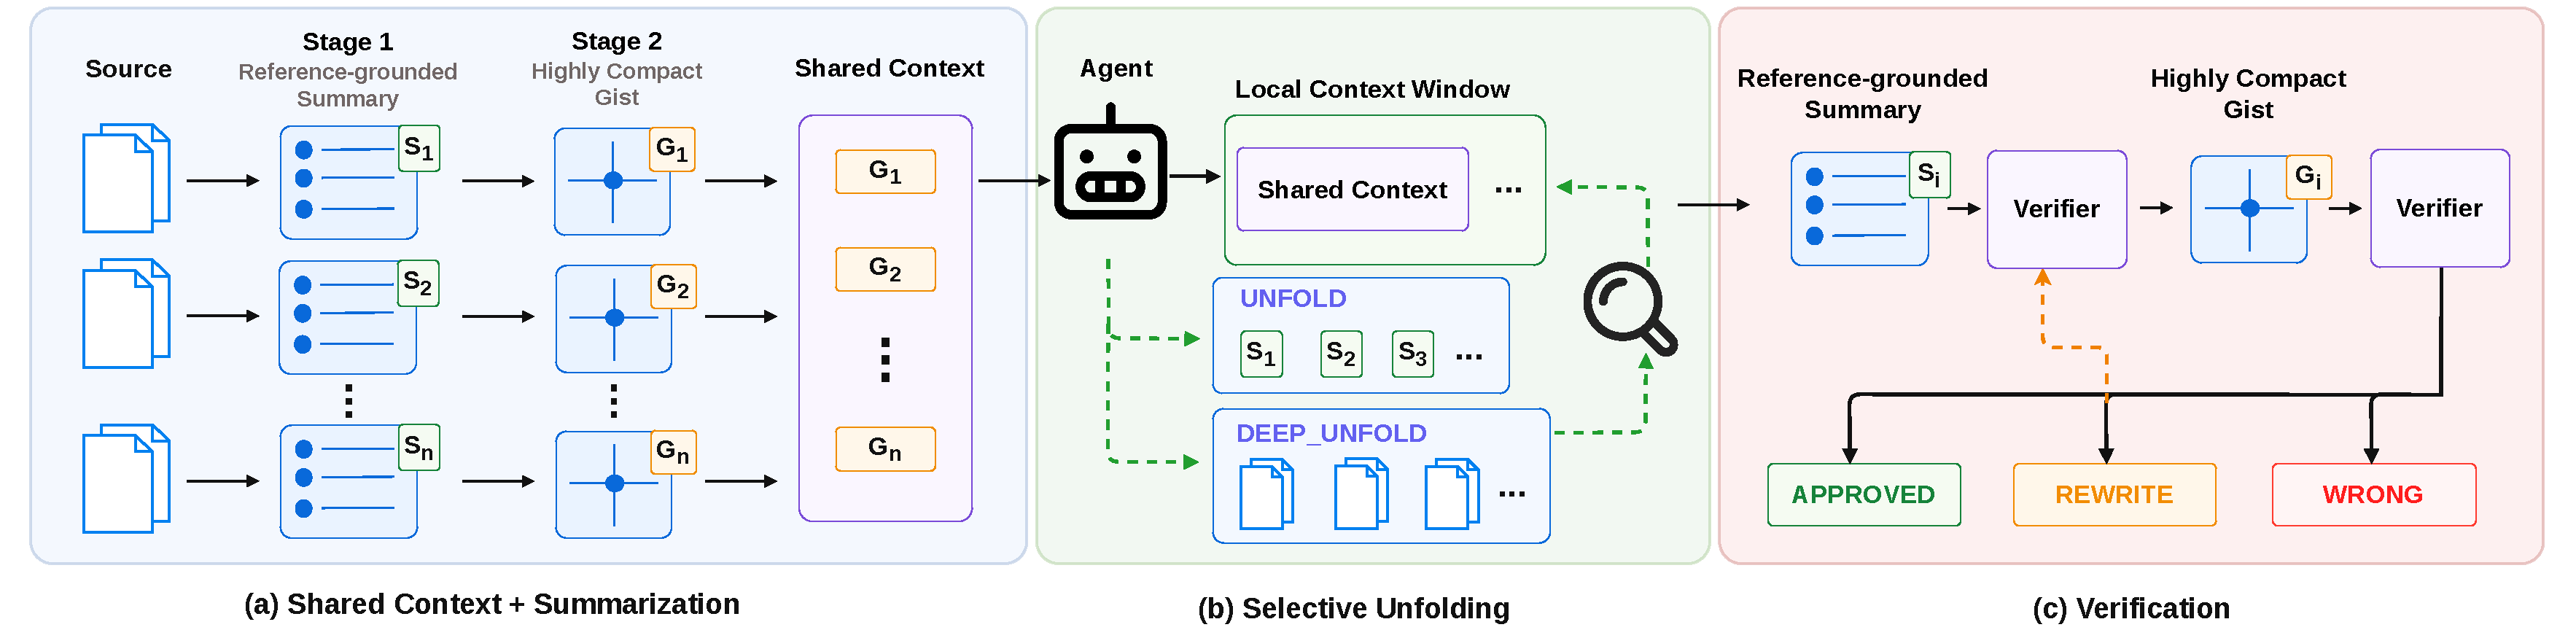
\includegraphics[width=1\linewidth]{modular.pdf}
    \caption{(a) Long source units are compressed into reference-grounded summaries $S_i$ and then compact gists $G_i$ stored in the shared context. (b) Agents read gists by default, selectively unfold them to summaries or raw evidence when needed, and (c) admit entries only after verification.}
    \label{fig:shared_context}
\end{figure}

\section{Method Details}

\subsection{Hierarchical Summarization}
\label{sec:summarization}
For long source units $r_i$ with label $\ell_i$, \toolName{} uses a three-level representation, $r_i \rightarrow S_i \rightarrow G_i$. The shared context $\sctx$ stores only compact gist entries $(\ell_i, G_i)$, giving every agent a lightweight global view of the corpus. The detailed backing content is stored outside $\sctx$: $\Lsto[\ell_i]$ contains the reference-grounded summary $S_i$, and $\Rsto[\ell_i]$ contains the corresponding raw source unit.

This hierarchy avoids relying on a lossy gist to directly select raw evidence while also avoiding broad raw-context unfolding. Agents first reason over gists, then unfold to $S_i$ or raw evidence only when finer-grained support is needed. For reasoning trajectories, \toolName{} usually admits a direct gist $G_i$, since later agents typically need the distilled finding, failure, feedback, or constraint rather than the full trace; the original trajectory remains available in $\Rsto[\ell_i]$ when needed.

We now describe the hierarchical summarization path for long source units.

\paragraph{Stage 1: $S_i$ (ref-grounded evidence map).}
Given a source unit $u_i$, the first-stage summarizer $\phi_1$ produces an evidence map consisting of a set of short bullets, each expressing a single atomic claim. Every bullet includes a {ref-tag} that identifies its supporting span in the raw text:
\begin{equation}
    \texttt{[ref: } h \;\ldots\; t\,\texttt{]},
\end{equation}
where $h$ and $t$ denote the first and last $N \geq 5$ words of the supporting span, respectively, copied verbatim. Formally,
\begin{equation}
    S_i = \phi_1(u_i;\, Q) = \{(b_{i,k},\, \reftag_{i,k})\}_{k=1}^{m_i}, \quad \reftag_{i,k} = (h_{i,k}, t_{i,k}),
\end{equation}
where $b_{i,k}$ is the $k$-th bullet and $\reftag_{i,k}$ is its ref-tag. $\phi_1$ is conditioned on the question $Q$ so that question-relevant content is extracted at higher fidelity. Full coverage of the source unit is required, as any portion may contain the critical evidence needed to answer the question. The resulting $S_i$ is stored in $\Lsto[\ell_i]$, with each bullet addressable by its local index $k$.

% The ref-tag mechanism makes Stage 1 verifiable: each concrete claim is explicitly grounded in a source span, enabling efficient validation without re-reading the full raw content.

\paragraph{Stage 2: $G_i$ (compact shared-context entry).}
A second-stage summarizer $\phi_2$ compresses $S_i$ into a short, highly compact gist:
\begin{equation}
    G_i = \phi_2(S_i;\, Q).
\end{equation}
This gist captures the relevance of $u_i$ to the query at a density that allows downstream agents to decide, at a glance, whether further inspection is needed. Only $G_i$ is admitted to $\sctx$, while $S_i$ and the raw content remain in $\mathcal{L}$ and $\mathcal{R}$ and are accessed only through selective unfolding (\S\ref{sec:unfold}).

% \yuzhen{Add the LLM-assist split boundaries strategy, and the coverage guarantee. Also introduce using cheap model for large corpus compression, with reference}

% \begin{figure}[!t]
%     \centering
%     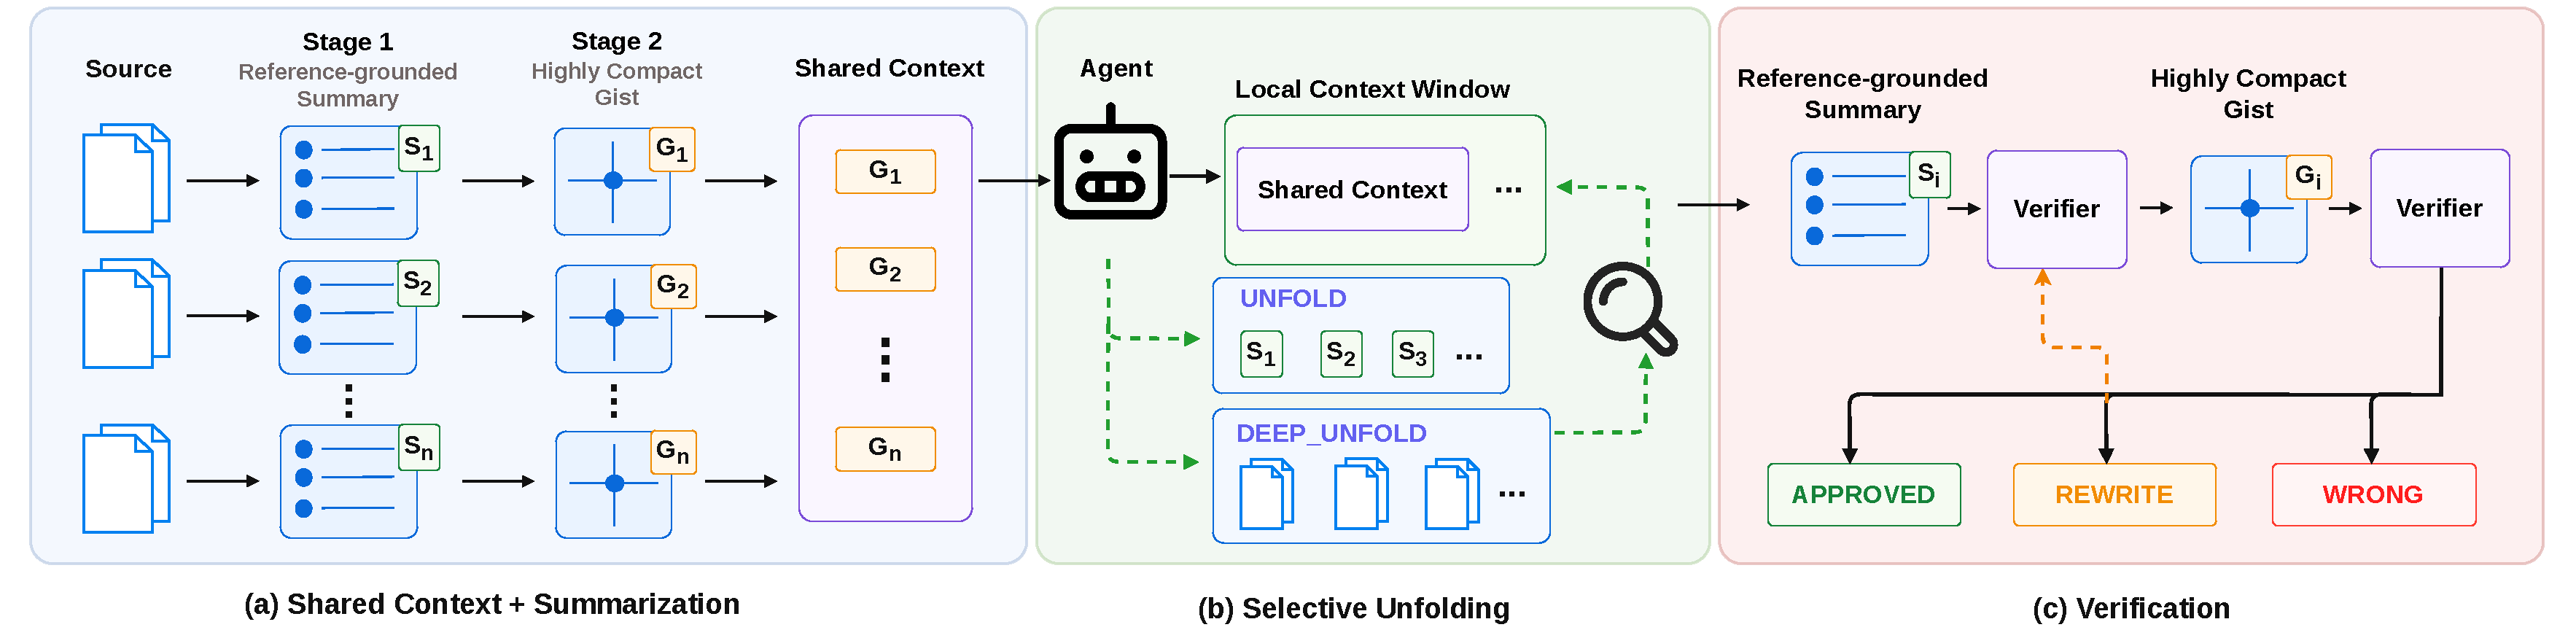
\includegraphics[width=1.0\linewidth]{modular.pdf}
%     \caption{Three core modules of \toolName{} (illustrated using the source-unit case). {(a) Shared Context + Summarization:} each source is summarized hierarchically into a reference-grounded summary $S_i$ and a compact gist $G_i$; only $G_i$ is admitted to the shared context. {(b) Selective Unfolding:} agents reason over the shared context by default and progressively unfold relevant entries to $S_i$ (\texttt{UNFOLD}) or to raw sources (\texttt{DEEP\_UNFOLD}) on demand. {(c) Verification:} both $S_i$ and $G_i$ are validated against their underlying evidence and routed to one of three outcomes: \textsc{Approved}, \textsc{Rewrite}, or \textsc{Wrong}.}
%     \label{fig:modular}
% \end{figure}

\subsection{Selective Unfolding}
\label{sec:unfold}
Agents reason over the shared context $\sctx$ by default, using the compact $G_i$ entries. When additional detail is required, they invoke {selective unfolding}, a coarse-to-fine, opt-in mechanism for retrieving more detailed information on demand. We implement unfolding in two stages: first, from $G_i$ to the reference-grounded summary $S_i$, and then, if necessary, from $S_i$ to the raw source content.

% \yuzhen{Hierarchical, coarse to fine search, Make sure both broad and deep requirement, Include neighborhood and also consider the coverage. Hybrid gist and summary search combination}

\paragraph{Stage 1: $G \rightarrow S$ (\texttt{UNFOLD}).}
At any reasoning step, the agent may request a small set of labels via an \texttt{UNFOLD: $\ell_1, \ell_2, \ldots$} directive. The orchestrator retrieves the corresponding $S_i$ summaries $\Lsto[\ell]$ and inlines their bullet-level evidence maps into the agent’s prompt for that call. This enables the agent to reason over grounded evidence rather than compressed gists.

\paragraph{Stage 2: $S \rightarrow \text{raw}$ (\texttt{DEEP\_UNFOLD}).}
After reasoning over the $S_i$ summaries, the agent may determine that finer-grained detail is required---for example, to resolve subtle qualifiers or verify exact wording. It can then emit a \texttt{DEEP\_UNFOLD: $\ell_1, \ldots$} directive specifying the labels whose raw content is needed. The orchestrator issues a follow-up call that combines the original task, the shared context $\sctx$, the previously unfolded summaries $S_i$, and the newly requested raw content from $\mathcal{R}$.

Unfolding proceeds in a coarse-to-fine, on-demand manner and may span multiple rounds up to a fixed limit, with each round allowing the agent to request additional $S_i$ or raw content as needed. Additionally, raw retrieval is also neighborhood-aware: requesting sub-chunk $n$ returns $n{\pm}1$ as well, which helps absorb off-by-one citation errors. Importantly, unfolded content is local to the requesting call and is not written back to the shared context $\sctx$, so subsequent agents still observe only the gist layer. This design prevents detailed intermediate content from polluting the shared context while preserving access to fine-grained evidence when necessary. As a result, the cost of detailed inspection scales with the amount of information actually required, rather than the total volume of available context.

\subsection{Admission-Time Verification}
\label{sec:verification}
Verification follows the compression path. For a reasoning trajectory, \toolName{} checks whether the gist $G_i$ faithfully preserves the relevant finding, failure, feedback, or constraint from the original result $r_i$. For a long source unit, \toolName{} verifies both levels of the hierarchy, first grounding the Stage-1 summary $S_i$ in the raw source and then checking the Stage-2 gist $G_i$ against $S_i$.

Specifically, each Stage-1 bullet $b$ with a reference $(h,t)$ is accepted only if the head $h$ and tail $\tque$ both appear, in order and verbatim, in the underlying source unit $u$. Bullets that fail this condition are routed to a targeted rewrite step, which either supplies a valid reference or drops the claim.

After this gate, an {iterative coverage loop} identifies large uncovered regions, defined as contiguous spans not referenced by any admitted bullet, and requests additional bullets for each gap. Newly generated bullets must pass the same reference and semantic-support checks before being added to $S_i$. The loop terminates when no large gaps remain or a fixed iteration limit is reached.

The Stage-2 gist $G_i$ is then produced from the verified $S_i$. Because $S_i$ contains only grounded claims, $G_i$ inherits this grounding at a coarse level. To guard against abstraction errors, $G_i$ undergoes a lightweight verification step using a cheaper LLM, such as DeepSeek-V4-Flash, which checks for hallucinations, semantic drift, and missing critical qualifiers relative to $S_i$. Only gists that pass this check are admitted to $\sctx$; otherwise, the update is rejected, regenerated, or returned to the task queue $\mathcal{T}$ with a rejection reason, up to a fixed retry limit.

% The verifier returns one of three outcomes: \textsc{Approved}, \textsc{Rewrite}, or \textsc{Wrong}. In the first two cases, a corrected and verified summary is produced and admitted as $G$. In the \textsc{Wrong} case, the task is returned to the task queue $\mathcal{T}$ with rejection reason, up to a fixed retry limit. As a result, every entry admitted to the shared context has passed an explicit grounding check and retains a traceable link to its supporting evidence. Because each $G$ entry preserves an addressable path through $S$ to its source ($u$ or $\Rsto$), any agent can later re-audit a suspect entry by traversing $\mathcal{L}$ and $\mathcal{R}$. Verification thus serves not only as an admission-time gate but also as a mechanism for on-demand re-grounding.

\subsection{Parallel Execution and Systems Optimizations}
\label{sec:orchestration}
\toolName{} uses three lightweight mechanisms to support safe and efficient
parallel execution: concurrent admission with disciplined reads and writes, a dependency-aware task queue, and KV-cache reuse across calls.

\paragraph{Concurrent admission and read/write discipline.}
Compression and verification are parallelized across completed results. Each finished agent independently proposes an update from its local result $r_i$, and the corresponding summarization and verification calls can run concurrently. The only synchronized step is admission. Once an update passes verification, \toolName{} first writes its backing content to $\mathcal{L}$ and $\mathcal{R}$, and then appends the visible entry $(\ell_i, G_i)$ to $\sctx$ through an atomic write. Agents read lock-free snapshots of $\sctx$ at dispatch time; entries committed later become visible only on the next snapshot.This write-before-publish ordering ensures that every visible label can be unfolded without a race, that later agents observe only fully verified entries, and that slow summarization or verification calls do not impose a global synchronization barrier.

\paragraph{Dependency-aware task queue.} At the beginning, given an input task $D$, \toolName{} first constructs a task topology: a numbered list in which each task is annotated with a $[\texttt{deps}: \ldots]$ tag specifying its upstream dependencies. Tasks with no dependencies are dispatched first; subsequent tasks become eligible as their dependencies complete. and subsequent tasks become eligible once their dependencies complete.
When the queue is exhausted, a single agent acquires a queue lock and invokes \textsc{GenerateMoreSubtasks} with the current shared context $\sctx$, the original plan, and the list of executed tasks. The function may return $[\textsc{Done}]$ if the original plan has been completed and no further unfolding is expected to change the state of any sub-claim. This step also prevents dependency deadlock in practice: when no pending task is eligible, the system does not wait indefinitely, but invokes \textsc{GenerateMoreSubtasks} to create missing prerequisite subtasks, revise blocked dependencies, or terminate if the current shared context is sufficient.

\paragraph{KV-cache reuse from a stable shared context.}
The shared-context design also improves KV-cache reuse. Because $\sctx$ is largely stable and accumulative, and consistently placed at the
beginning of each model invocation, it forms a persistent prefix across calls. This is useful in multi-step reasoning, where many LLM calls share the same global state but differ only in the task-specific suffix. As a result, repeated computation over the shared prefix can be amortized, yielding larger efficiency gains as the number of reasoning steps grows.


% \paragraph{Shared-context cleanup.} 
% An optional context-cleanup pass is performed before each replanning step: the model is prompted to identify entries that are mutually contradictory or exact duplicates of other entries, and flagged entries are removed from $\sctx$ prior to replanning. This not only enforces global consistency, but also keeps the reasoning trace clean by pruning the residue of useless intermediate trials that would otherwise distract downstream agents from the main line of reasoning. Because the cleanup is invoked at most once per replanning boundary, its computational cost remains bounded. In addition, to prevent the shared context from overflowing the model's context window, the cleanup pass is also triggered whenever the total token count of $\sctx$ exceeds a threshold.



\end{document}
